\documentclass[12pt,a4paper]{article}
\usepackage{fix-cm}
\usepackage{setspace}
\usepackage{fancyhdr}
\usepackage{lettrine}
\usepackage{geometry}
\usepackage[english]{babel}
\usepackage[utf8]{inputenc}
\usepackage{dcolumn}
\usepackage{array,booktabs,ragged2e}
\usepackage{pgfplots,pgfplotstable,pgfkeys,filecontents}
\usepackage{csvsimple,ifthen,etoolbox}
\usepackage{amsmath,latexsym}
\usepackage{gensymb}
\usepackage{amssymb}
\usepackage{amsmath}
\usepackage{tikz}
\usepackage{xfrac}
\usepackage{fancyhdr}
\usepackage{lettrine}
\usepackage{geometry}
\usepackage{dcolumn}
\usepackage[htt]{hyphenat}
\usepackage{circuitikz}
\usepackage{siunitx}
\usepackage{nicefrac}
\usepackage{hyperref}
\usepackage{xurl}
\usepackage{color,soul}
\usepackage{titlesec}
\usepackage[T1]{fontenc}
\usepackage{adjustbox}
\usepackage{pdfpages}
\usepackage{multirow}
\usepackage{graphicx}
\usepackage{wrapfig}
\usetikzlibrary{fit}
\usepackage{float}
\usepackage{rotating}
\usepackage{pdflscape}
\usepackage{caption}
\usepackage{subcaption}
\usepackage{mathtools}
\usepackage{upgreek}
\usepackage[toc,page]{appendix}
\usepackage[section]{placeins}

% --- Float placement: keep figures near their references ---
\setcounter{topnumber}{4}
\setcounter{bottomnumber}{4}
\setcounter{totalnumber}{6}
\renewcommand{\topfraction}{0.9}
\renewcommand{\bottomfraction}{0.9}
\renewcommand{\textfraction}{0.05}
\renewcommand{\floatpagefraction}{0.8}

\newcommand\addvmargin[1]{
	\node[fit=(current bounding box),inner ysep=#1,inner xsep=0]{};
}
\geometry{
	a4paper,
	total={8.5in,11in},
	left=1in,
	right=1in,
	top=1in,
	bottom=1in,
}

\pagestyle{fancy}
\setlength{\headheight}{28pt}

\raggedbottom
\newcolumntype{R}[1]{>{\RaggedLeft\arraybackslash}p{#1}}
\renewcommand{\baselinestretch}{1.4}
\setlength\parindent{0pt}
\def\doubleunderline#1{\underline{\underline{#1}}}

\newcommand{\reporttitle}[3][ ]{
	\thispagestyle{empty}
	\begin{center}
		\vspace*{8mm}
		\fontshape{sc}
		\fontsize{17pt}{20pt}
		\selectfont
		#2
		\linebreak
		\fontsize{25pt}{25pt}
		\bfseries
		\selectfont
		#3
		\linebreak
		\fontshape{n}
		\fontsize{15pt}{25pt}
		\normalfont
		\selectfont
		#1
	\end{center}
}

% Header ============================================================================================
\pagestyle{fancy}
\fancyhf{}
\lhead{Master's Thesis\\IPA / Quanz Group}
\renewcommand{\sectionmark}[1]{\markboth{#1}{}}
\chead{July 2026\\ \nouppercase{\leftmark}}
\rhead{FS 26\\Nicolas Feuchthofen}
\cfoot{Page \thepage}

\fancypagestyle{chapteropening}{
    \fancyhf{}
    \cfoot{Page \thepage}
    \renewcommand{\headrulewidth}{0pt}
}

\definecolor{lifeaccent}{HTML}{76232F}
\definecolor{lifepale}{HTML}{E9E4E5}
\definecolor{lifegray}{HTML}{727272}

\newif\ifappendixchapter
\appendixchapterfalse

\newcommand{\chapteropening}[2]{%
    \clearpage
    \refstepcounter{section}%
    \sectionmark{#1}%
    \addcontentsline{toc}{section}{\protect\numberline{\thesection}#1}%
    \thispagestyle{chapteropening}%
    \begin{tikzpicture}[remember picture,overlay]
        \fill[lifeaccent]
            ([xshift=24mm,yshift=-28mm]current page.north west)
            rectangle
            ([xshift=28mm,yshift=-105mm]current page.north west);
        \node[
            anchor=base east,
            text=lifepale,
            font=\fontsize{72}{72}\selectfont\bfseries
        ] at ([xshift=-20mm,yshift=-35mm]current page.north east) {\thesection};
    \end{tikzpicture}%
    \vspace*{26mm}
    \hspace*{13mm}%
    \begin{minipage}{0.82\textwidth}
        {\color{lifeaccent}\fontsize{10}{12}\selectfont\bfseries\scshape
        \ifappendixchapter Appendix\else Chapter\fi~\thesection}

        \vspace{7mm}

        {\hyphenpenalty=10000\exhyphenpenalty=10000
        \RaggedRight\fontsize{32}{36}\selectfont\bfseries #1\par}

        \vspace{7mm}

        {\color{lifegray}\RaggedRight\large #2\par}
    \end{minipage}\par

    \vspace{28mm}
    \noindent\ignorespaces
}

%\setlength{\columnsep}{5mm}
%\setlength{\columnseprule}{0.5pt}
\setlength{\parindent}{0pt}
\renewcommand{\baselinestretch}{1.4}
\setlength{\parskip}{3mm}
% ===============================================================================================================

\onehalfspacing

\numberwithin{equation}{section}
\numberwithin{figure}{section}
\numberwithin{table}{section}

\begin{document}
% Titel ========================================================================================================
\reporttitle[\vspace{-1.5cm} \\ \rule{6.4cm}{0.4pt} \\ \vspace{-0.5cm} \textit{Nicolas Feuchthofen} \\ Supervisors: Dr. Felix Dannert, Prof. Dr. Sascha Patrick Quanz\\ \vspace{-0.4cm} July 2026]{Master's Thesis}{Instrument-Agnostic Iso-Mission-Time Noise Budgets for LIFE Using a Null-Order Proxy}

\vspace{1cm}

\begin{figure}[htp]
    \centering
    
\includegraphics[width=0.5\linewidth]{images/LIFE_Logo_Wordmark_Primary_Digital_RBG-Black.png}
\end{figure}

\vspace{1cm}

\newpage

\begin{abstract}
    The Large Interferometer For Exoplanets (LIFE) aims to detect and characterize nearby terrestrial exoplanets in the mid-infrared. Its scientific return depends on how much additional instrumental random noise can be tolerated without making the required observing program too long. This thesis develops an Agnostic Mission Simulator (AMS) and a trade-space explorer that convert a wavelength-dependent aggregate random-noise allowance into a 90th-percentile mission time. The source calculation was reformulated analytically for circularly symmetric astrophysical backgrounds, eliminating the former spatial pixel grid, correcting the local-zodiacal normalization by about 27\%, and permitting accurate wavelength-bin quadrature. The AMS reproduces the shared LIFEsim source-model SNRs to floating-point precision.

    Final calculations compare three additive budget shapes---flat, short-weighted, and long-weighted---for the Hab2Max and Hab2Min catalogs at limiting magnitude 7, field of regard $65^\circ$, and 12\,h slew time. For the second-order double-Bracewell reference, the short-weighted ramp admits the largest endpoint, consistent with geometric stellar leakage dominating the short-wavelength variance. In the fourth-order proxy, stellar leakage is suppressed by three to five orders of magnitude and the ordering reverses: zodiacal backgrounds dominate and the long-weighted ramp admits the largest endpoint. At the primary mission-time targets, the flat allowance rises from 140 to 640\,ph\,s$^{-1}$\,$\upmu$m$^{-1}$ for Hab2Max at 5.5\,yr and from 65 to 590\,ph\,s$^{-1}$\,$\upmu$m$^{-1}$ for Hab2Min at 7.5\,yr when changing from null order two to four.

    These values are iso-mission-time amplitudes within tested budget families, not wavelength-by-wavelength subsystem requirements. The null-order comparison uses an unnormalized $\sin^n$ transmission proxy with fixed collecting area, efficiency, and baseline prescription; it therefore measures the impact of the modeled null order and its associated throughput change rather than predicting a concrete fourth-order LIFE architecture. Charging that proxy the optical efficiency penalty of a realizable four-aperture fourth-order combiner removes every admissible allowance at the targets studied, because the mission time required with no added noise already exceeds them. Across catalogs and null orders the required time scales with the inverse of throughput, tempered by a slew-dominated fraction of 17 to 29\% that does not scale at all, and the cost of halving the efficiency exceeds the benefit of the deeper null by a factor of three to five.
\end{abstract}

\newpage

% ===============================================================================================================

\tableofcontents

\chapteropening{Introduction}{Why LIFE matters and how a science goal becomes an instrument requirement} \label{sec: introduction}
Human curiosity extends far beyond Earth. We seek to understand how life began and whether Earth is its only home in the Galaxy. The Large Interferometer For Exoplanets (LIFE) turns that broad question into a concrete observational program: detecting nearby temperate terrestrial planets in the mid-infrared, measuring their thermal spectra, and using those measurements to constrain planet populations, atmospheric composition, and possible habitability \cite{quanz2022life1,konrad2022life3}.

For me, this scientific promise makes the practical definition of LIFE especially consequential. A mission can deliver those measurements only if its instrument can be built and operated within credible performance limits. This project therefore asks how much aggregate instrumental random noise LIFE can tolerate, and where in wavelength that noise is least damaging, before the required observing program becomes too long. Answering that question helps define instrument boundaries, test the feasibility of the approach, and increase confidence in both the mission concept and the conclusions drawn from its measurements.

The reference LIFE studies used here establish the astrophysical source model, signal extraction, and expected detection and characterization performance for a double-Bracewell interferometer \cite{quanz2022life1,dannert2022life2,dannert2025thesis}. An aggregate instrumental random-noise term is not itself new, and Section \ref{sec: intro: prior work} records what this work inherits. What the reference studies do not provide is its inversion: the wavelength-dependent \textit{iso-mission-time} boundary, that is, the set of noise-budget amplitudes that all lead to the same required mission time, for a mechanism-independent aggregate random-noise term. This thesis fills that narrower gap with two linked tools. The \textit{Agnostic Mission Simulator} (AMS) maps a specified noise budget and operating point to mission time; the \textit{Trade Space Explorer} (TSE) inverts that mapping to find the largest tolerated budget amplitude. A controlled change from a second- to a fourth-order transmission proxy then moves the spectral region that tolerates the most added noise from short to long wavelengths. The direction of that change follows from the known suppression of geometric stellar leakage at a deeper null; what the completed exploration establishes is that the reversal survives the full nonlinear scheduling and percentile chain, and that it holds under equal integrated added noise rather than only under equal ramp endpoints.

This work keeps the double Bracewell as its reference geometry. It is mechanism-agnostic only for an aggregate random-noise allowance: individual independent random terms are represented by their common equivalent rate. The result is therefore a bridge quantity. It translates a science-level completion time into an allowed single-output random count rate at a defined \textit{pre-efficiency reference plane}. That plane is the point in the signal chain at which photon rates have been multiplied by the collecting area but not yet by the optical throughput or the detector quantum efficiency, so a rate quoted there is independent of how those two factors are eventually apportioned; Section \ref{sec: intro: params} fixes it precisely. A later engineering allocation can map detector, optical, thermal, and control-noise terms to that plane and test their combined variance against the allowance. This thesis does not perform that subsystem allocation and cannot decide which hardware implementation is easiest. Architecture dependence is parameterized only through the explicitly limited null-order proxy, not through an arbitrary-architecture simulation.

\subsection{Research Questions} \label{sec: intro: research questions}
This thesis addresses the following central question.

\textit{For a specified operating point and a tested family of additive random-noise budgets, what maximum budget amplitude is compatible with completing Experiment~1---the inherited detection-and-characterization program for 50 qualifying catalog planets---within a chosen mission-time target?}

This question is structured into the following sub-questions:
\begin{itemize}
    \item \textit{What is the dimension of the AMS parameter space?}
    \item \textit{Which source-model computations can be reused when only global filters or tested budget amplitudes change?}
    \item \textit{Can we reduce the AMS parameter space without significantly compromising fidelity?}
    \item \textit{Can we locate the maximum tolerated amplitude for flat and linear-ramp random-noise budgets at a fixed operating point?}
    \item \textit{How does changing the null order represented by the transmission proxy alter the tolerated spectral budget shapes?}
\end{itemize}

\subsection{Relation to Prior Work} \label{sec: intro: prior work}
The tools and the source model used here are inherited, so it is worth stating precisely what is taken over and what is added. LIFE paper II supplies the double-Bracewell response, the signal-extraction formalism, and the LIFEsim source model on which the simulator in Section \ref{sec: methods: AMS} is built, and its appendix constrains instrumental perturbations mechanism by mechanism \cite{dannert2022life2}.

The direct predecessor is Dannert's doctoral thesis \cite{dannert2025thesis}. It already introduces an aggregate instrumental photon-noise term that collects all additional photon-noise contributions, defines a fundamental-noise-limited criterion comparing that term against the astrophysical floor, and studies the resulting effect on detection yield. The aggregate random-noise quantity used here is therefore not a new object, and the present work does not claim it as one. What is new is the direction in which the mapping is used. Where the predecessor propagates an assumed instrumental noise level forward to a yield, this thesis fixes the science outcome---Experiment 1 completed within a stated mission-time target---and inverts for the largest random-noise amplitude compatible with it, resolved in wavelength across a tested family of budget shapes.

Two earlier master's theses in the same programme occupy neighbouring ground. Norbruis \cite{norbruis2023} built a LIFEsim-derived performance model, used P-Pop populations as a test set, and ran grid and multi-objective optimisation over array geometry, aperture area, and instrument temperature to produce Pareto fronts against a detection figure of merit. That work optimises the design for yield; the present work holds the design fixed and solves for a tolerated noise allowance at fixed mission time. Binkert \cite{binkert2023} addresses signal extraction and molecular-feature detection during the search phase, a different layer of the same mission and without overlap with the question asked here.

Against that background, three things in this thesis are new: the iso-mission-time inversion itself, the closed-form treatment of the circularly symmetric backgrounds that removes image size as a production-science parameter (Section \ref{sec: ts reduction: image spec}), and the finding that the spectral preference between budget shapes inverts with null order and survives the full scheduling and percentile chain rather than only the underlying leakage scaling.

The remainder follows the causal chain from mission goal to engineering requirement. Section \ref{sec: background} establishes the experiment, target populations, measurement, SNR, and error budget. Section \ref{sec: methods} builds the fixed-reference simulator and null-order proxy. Section \ref{sec: ts reduction} reduces the raw trade space and derives the analytic background response. Section \ref{sec: tse} then presents the completed exploration, first at the nominal second-order null and then at fourth order. The discussion and conclusion state what the resulting allowances do and do not imply for LIFE.

\chapteropening{Background and Procedures}{From a synthetic planetary population to a measurable mission signal} \label{sec: background}
This project is conducted within the scope of the LIFE space mission. To connect its scientific objective to an engineering requirement, we first need to establish what the experiment asks the instrument to observe and how those observations become a mission-time calculation. LIFE is a proposed space-based mid-infrared nulling interferometer for detecting and characterizing nearby temperate terrestrial planets \cite{quanz2022life1,dannert2022life2}. Its current concept separates light collection from beam combination: four free-flying collector spacecraft feed a central beam-combiner spacecraft while the formation rotates about the line of sight. The long effective baseline supplies angular resolution that a single space telescope of comparable total collecting area could not provide.

The scientific reason for observing in the mid-infrared is twofold. A temperate planet emits much of its thermal radiation in this range, reducing the star--planet contrast relative to visible reflected light, and several atmospheric molecules have diagnostically useful absorption bands there. Nulling interferometry does not form a conventional resolved image of every system. Instead, it suppresses the on-axis star, modulates off-axis emission through rotation, and measures a wavelength-dependent differential signal. Detecting that signal constrains planet populations; accumulating a spectrum can constrain atmospheric composition. The latter remains an inference problem rather than an automatic identification of life \cite{quanz2022life1,konrad2022life3}.

This thesis retains the four-aperture double-Bracewell response used by LIFEsim \cite{dannert2022life2}. Two aperture pairs first produce destructive and constructive outputs. The destructive outputs are recombined with a relative phase shift to produce two chopped dark outputs whose difference changes sign for an off-axis source. The reference response has a second-order intensity null: close to the optical axis, transmitted stellar intensity grows quadratically with angular offset. Figure \ref{fig: double-bracewell-layout} shows this optical logic.

\begin{figure}[htbp]
    \centering
    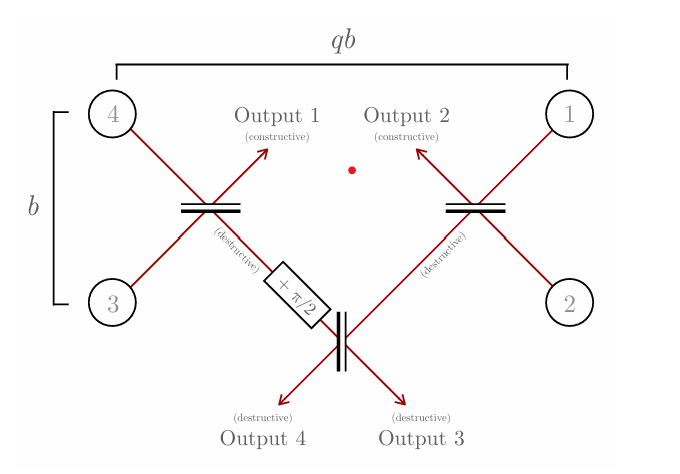
\includegraphics[width=0.8\linewidth]{images/intro/dannert2022-double-bracewell-layout.png}
    \caption{Double-Bracewell interferometer layout reproduced from Dannert et al. \cite{dannert2022life2}. Light from apertures 4 and 3, and from 1 and 2, is combined to form destructive and constructive outputs. The destructive outputs are recombined with a relative phase shift of $\pi/2$ to form two chopped dark outputs with a second-order null.}
    \label{fig: double-bracewell-layout}
\end{figure}

\newpage

\subsection{The Experiment and Assumptions}
This work adopts the legacy LIFEsim/AMS configuration called \textit{Experiment 1}: the mission must detect and characterize 50 catalog planets with radii between 0.5 and 1.5 Earth radii, host-star temperatures between 4370 and 7310\,K, and a positive catalog habitable-zone flag. The thresholds and instrument settings used throughout the completed data collection are summarized in Table \ref{tab: study assumptions}. They define this study's controlled comparison; they should not be read as a claim that every value is the latest top-level LIFE mission requirement.

\begin{table}[htbp]
\centering
\begin{tabular}{@{}p{0.35\linewidth}p{0.21\linewidth}p{0.34\linewidth}@{}}
\toprule
Quantity & Adopted value & Role in the calculation \\
\midrule
Qualifying sample & 50 planets & Experiment-completion target \\
Planet radius & $0.5$--$1.5\,R_\oplus$ & Catalog eligibility filter \\
Host temperature & 4370--7310\,K & Catalog eligibility filter \\
Habitable zone & Catalog flag required & Catalog eligibility filter \\
Detection threshold & SNR 7 & Common detection campaign \\
Characterization threshold & SNR 44.1 & Broadband characterization proxy \\
Orbit epochs & 5 & Detection plus four follow-up visits \\
Collector diameter & 4\,m each & Photon collecting area \\
Optical throughput & 0.15 & Pre-detector transmission \\
Quantum efficiency & 0.60 & Photon-to-count conversion \\
Total efficiency & 0.09 & Product of throughput and quantum efficiency \\
Spectral band and resolution & 4--18.5\,$\upmu$m, $R=20$ & 31 finite wavelength bins \\
Baseline ratio and bounds & $r=6$, 10--100\,m & Imaging/nulling geometry and clipping \\
\bottomrule
\end{tabular}
\caption{Fixed LIFEsim/AMS settings used for all final simulations. SNR 7 follows the LIFE yield-study detection convention \cite{kammerer2022life6}. The characterization value 44.1 is the integrated broadband equivalent of a legacy per-channel requirement of SNR 10 at $11.2\,\upmu$m and $R=50$ \cite{dannert2025thesis}.}
\label{tab: study assumptions}
\end{table}

The characterization threshold deserves particular care. It is not a universal statement that every molecular feature is measurable at bulk SNR 44.1. It is a retained broadband proxy that permits a consistent mission-time comparison with the inherited simulation framework \cite{dannert2025thesis}. Similarly, the fixed 4\,m collectors and 9\% total efficiency set photon rates but are not optimized in this thesis. The output is conditional on all these assumptions.

These assumptions specify the required scientific outcome, but not the individual planets that must supply it. We therefore next define the simulated target populations on which the mission-time calculation is based.

\subsection{Target Catalog Selection} \label{sec: intro: catalog}
The LIFE target catalogs are created from a common scaffold of 4505 nearby stars, including Sun-like and M-dwarf hosts out to roughly 50\,pc. This scaffold was inherited together with the catalogs; its entries carry TESS Input Catalog identifiers, and the star count and distance limit quoted here were verified directly from the catalog files rather than taken from a published target list. It is deliberately broader than the stellar sample of LIFE paper VI, which is restricted to single and wide binary main-sequence stars within 20\,pc \cite{kammerer2022life6}. The $\eta_{\oplus}$ values adopted in Table \ref{tab: eta earth} were averaged over that smaller sample, so the occurrence normalization and the stellar scaffold used here are not drawn from the same stellar population. This is acceptable for the present purpose, because the comparison throughout is between operating points and budget shapes evaluated on one fixed scaffold, but it means the absolute planet counts in Table \ref{tab: catalog inventory} should not be read against the yields reported in LIFE paper VI. Since planets are not known around most of them, the population must be synthesized. P-Pop draws occurrence and orbital properties constrained by Kepler statistics and places a hypothetical planetary system around every stellar target \cite{kammerer2018ppop}. One complete draw over the stellar scaffold is called a \textit{universe}. The 100 universes in a catalog are therefore alternative population realizations, not 100 independent observations of the real Galaxy.

We use two catalogs, \textit{Hab2Min} and \textit{Hab2Max}, with 100 universes each. They implement the lower and upper ``hab2 stars'' extrapolation scenarios of the Bryson et al.\ occurrence model as adopted in LIFE paper VI \cite{bryson2021occurrence,kammerer2022life6}. The quantity $\eta_{\oplus}$ is the average number of exo-Earth candidates per Sun-like star, not the fraction of stars hosting at least one such planet. Hab2Min represents the less favorable and Hab2Max the more favorable occurrence scenario; their difference is driven chiefly by the extrapolation beyond 500\,d, where Kepler completeness no longer directly constrains the occurrence surface. Both retain the same stars, so comparing them changes the hypothetical planets rather than the accessible stellar neighborhood. M dwarfs remain in the source catalogs but fail the Experiment~1 host-temperature cut and are not qualifying targets.

\begin{table}[htbp]
\centering
\begin{tabular}{@{}ll@{}}
\toprule
Catalog & $\eta_{\oplus}$ \\
\midrule
Hab2Min & $0.19_{-0.10}^{+0.19}$ \\
Hab2Max & $0.34_{-0.19}^{+0.38}$ \\
\bottomrule
\end{tabular}
\caption{Mean numbers of exo-Earth candidates per Sun-like star used to define the two occurrence scenarios \cite{bryson2021occurrence,kammerer2022life6}. The asymmetric bounds are the reported $1\sigma$ occurrence-model uncertainties and are dominated by occurrence-rate and long-period extrapolation uncertainty.}
\label{tab: eta earth}
\end{table}

\begin{table}[htbp]
\centering
\small
\begin{tabular}{@{}lrrrrr@{}}
\toprule
Catalog & Universes & Planet rows & Stars & Eligible planet rows & Eligible planets/universe \\
\midrule
Hab2Min & 100 & 486\,244 & 4505 & 205\,715 & 1958--2154 \\
Hab2Max & 100 & 729\,925 & 4505 & 318\,654 & 3049--3331 \\
\bottomrule
\end{tabular}
\caption{Inventory measured from the exact input files used in this work after loading them through the same P-Pop interface as the AMS. ``Eligible'' applies only the Experiment~1 radius, host-temperature, and habitable-zone filters; visibility, SNR, and scheduling cuts are applied later. The median eligible counts are 2058.5 for Hab2Min and 3194 for Hab2Max. LIFE paper VI uses a narrower exo-Earth-candidate subset, $0.8a_p^{-0.5}R_\oplus\leq R_p\leq1.4R_\oplus$, for its occurrence analysis; that definition does not replace the broader Experiment~1 radius filter used here \cite{kammerer2022life6}.}
\label{tab: catalog inventory}
\end{table}

The catalog ensemble has two roles. It exposes the scheduler to different possible planet populations, and it supplies the distribution from which the 90th-percentile mission time is taken. Catalog eligibility alone does not imply detectability: transmission, noise, magnitude, field of regard, and the finite observing campaign all act later. This distinction explains why target selection precedes signal collection in the narrative.

The catalog fixes the systems and planets to be observed; the next step is to determine how light from each hypothetical planet is separated from its much brighter surroundings.

\subsection{Signal Collection: Transmission Map, Chopping, and Modulation} \label{sec: intro: signal collection}
Before quantifying the SNR, we must establish how the interferometer separates an off-axis planet from bright backgrounds. A transmission map $T(\alpha,\beta)$ gives the fraction of incident flux reaching one output at sky offset $(\alpha,\beta)$. Following the notation of LIFE paper II, the nulling baseline $b$ sets the broad null envelope, while the imaging baseline $rb$ sets the fine chopping and modulation fringes; the baseline ratio is $r=6$ in the nominal settings. For each star, $b$ is selected using the habitable-zone-centre prescription and clipped to the instrument bounds. A common field-of-view taper attenuates off-axis light. The star lies on the central null, whereas an off-axis planet samples the surrounding fringes \cite{dannert2022life2}.

The two destructive outputs are chopped by subtraction. Their symmetric mean backgrounds cancel in the difference, but their independent photon-counting variances remain and add. A planet generally contributes to both outputs, but unequally, and therefore survives the subtraction (Fig. \ref{fig: transmission maps a}, right).

The final ingredient is \textit{modulation} through array rotation. Over an observation the entire array is slowly rotated about the line of sight. A planet at a fixed angular separation is thereby swept through the alternating positive and negative lobes of the chopped map, so that its contribution to the differential output oscillates in time, tracing out a characteristic \textit{transmission curve} as a function of rotation angle (Fig. \ref{fig: transmission maps b}). The symmetric backgrounds, being nearly axisymmetric, stay approximately constant under this rotation: Lay reports that the stellar and local-zodiacal geometric leakage rates are nominally independent of the array rotation angle and therefore appear at zero frequency, and Dannert et al. state correspondingly that for rotationally symmetric sources the detected signal does not depend on the rotation angle of the array \cite{lay2004systematic,dannert2022life2}. The planetary signal is therefore encoded as a time-modulated component riding on an essentially static background, which allows it to be isolated in subsequent analysis \cite{lay2005imaging,dannert2022life2}. This is the origin of the temporal average $\langle\cdot\rangle$ over one full array rotation that appears throughout the SNR derivation below.

The calculation does not simulate a time-series estimator sample by sample. It uses the root-mean-square response over a complete, uniformly sampled rotation. For a chopped planet transmission $m(\theta)=T_3(\theta)-T_4(\theta)$, the effective signal coefficient is therefore
\begin{align}
s=\left[\frac{1}{2\pi}\int_0^{2\pi}m^2(\theta)\,\mathrm{d}\theta\right]^{1/2}.
\end{align}
This is the matched-modulation amplitude for white, rotation-independent variance under the adopted normalization. A constant symmetric brightness cancels from the chopped mean, but it still sends photons to each output and therefore remains in the variance. Figure \ref{fig: transmission maps} shows the single-output and chopped maps over which these coefficients are averaged.

\begin{figure}[htbp]
    \centering
    \begin{subfigure}{\textwidth}
        \centering
        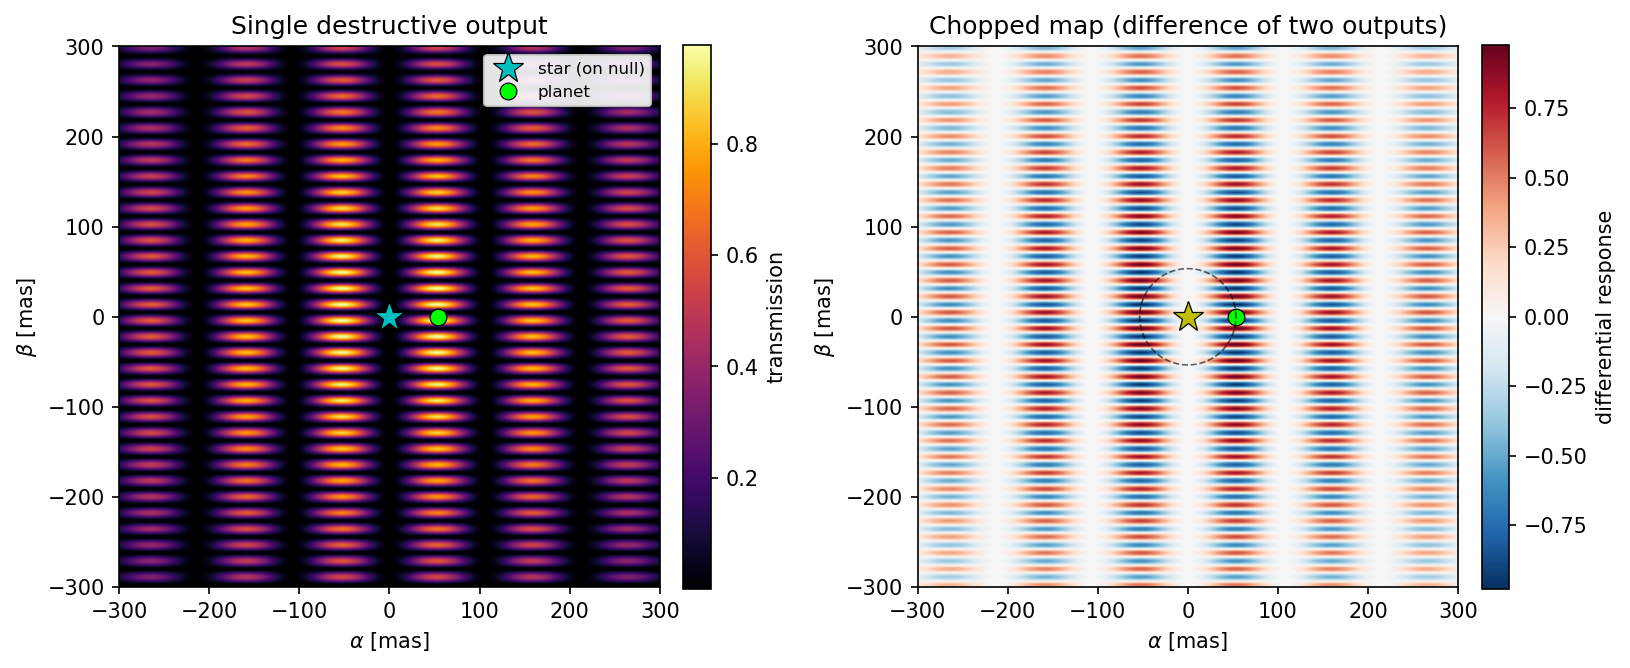
\includegraphics[width=\linewidth]{images/intro/transmission_maps.png}
        \caption{Transmission maps of the double Bracewell array.}
        \label{fig: transmission maps a}
    \end{subfigure}

    \vspace{2mm}

    \begin{subfigure}{.72\textwidth}
        \centering
        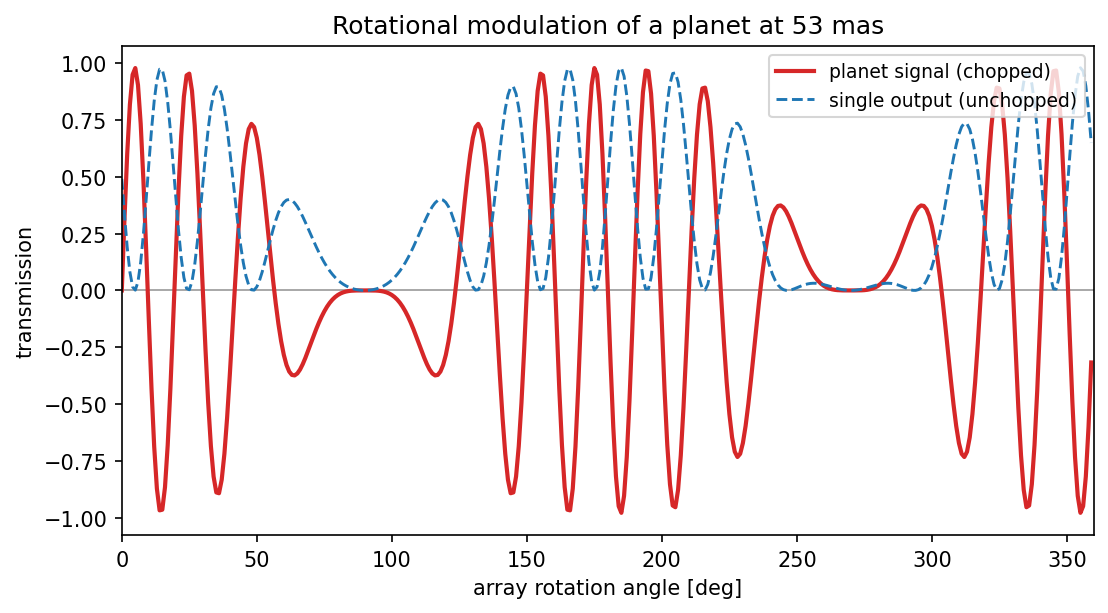
\includegraphics[width=\linewidth]{images/intro/transmission_modulation.png}
        \caption{Rotational modulation of the marked planet.}
        \label{fig: transmission maps b}
    \end{subfigure}
    \caption{Signal collection in the double-Bracewell reference geometry at $10.4\,\upmu$m, $b=20\,$m and nominal baseline ratio $r=6$, zoomed to the central $\pm300\,$mas. (a) A single destructive-output map and its chopped difference. Symmetric mean contributions cancel in the difference, whereas an off-axis planet generally has unequal transmission in the two outputs. (b) Rotation modulates the chopped planet signal; the unchopped single-output response used for its photon-noise term has a different weighting.}
    \label{fig: transmission maps}
\end{figure}

Two consequences of this scheme carry directly into the SNR. First, the planetary \textit{signal} is collected through the chopped map, whereas the planetary \textit{photon noise}, which is insensitive to the sign of the modulation, is collected through a single, unchopped output; the two therefore enter with different transmission weights. Second, because the map is integrated over a full rotation, the effective response becomes radially symmetric and depends only on the angular separation of the planet and on the nulling baseline. This rotation-averaged response, further attenuated by a field-of-view taper that models the loss of off-axis coupling into the instrument's optical fibers, is the \textit{transmission efficiency} introduced in Section \ref{sec: intro: params}. Having established what reaches the detector and how it is weighted, we can now quantify whether the planet can be distinguished from noise.

\subsection{The Signal-To-Noise Ratio (SNR)}
The SNR is the expected modulated count signal divided by the standard deviation of the associated random count fluctuation. The implementation evaluates finite wavelength bins. Its reference planes are easy to confuse because planet flux is naturally specified at the observer, whereas extended backgrounds have already been integrated over collecting area. Table \ref{tab: snr symbols} makes the convention explicit.

\begin{table}[htbp]
\centering
\begin{tabular}{@{}lll@{}}
\toprule
Symbol & Meaning at the SNR interface & Units \\
\midrule
$F_{p,i}$ & Planet photon flux at the collectors, integrated over bin $i$ & ph\,s$^{-1}$\,m$^{-2}$ \\
$A$ & Total effective collecting area in the source convention & m$^2$ \\
$\eta$ & Optical throughput times quantum efficiency & 1 \\
$s_i$ & RMS chopped planet-response coefficient & 1 \\
$n_i$ & RMS single-output planet-noise coefficient & 1 \\
$B_i$ & Single-output astrophysical rate after area, before $\eta$ & ph\,s$^{-1}$ \\
$N_{I,i}$ & Added single-output rate after area, before $\eta$ & ph\,s$^{-1}$ \\
$t$ & On-source integration time & s \\
\bottomrule
\end{tabular}
\caption{SNR symbols and reference-plane convention. The reported spectral budget $N_I(\lambda)$ is converted to a bin rate by $N_{I,i}=N_I(\lambda_i)\Delta\lambda_i$.}
\label{tab: snr symbols}
\end{table}

For bin $i$, the expected chopped planet counts follow from its incident flux, collecting area, efficiency, time, and RMS modulation response. Each destructive output is a Poisson stream. If the two output counts have means $\mu_3$ and $\mu_4$, then
\begin{align}
\mathrm{Var}(C_3-C_4)=\mathrm{Var}(C_3)+\mathrm{Var}(C_4)=\mu_3+\mu_4
\end{align}
when the streams are independent. Symmetric backgrounds have equal rotation-averaged rates in both outputs, so subtracting their means removes the DC signal but doubles their single-output variance. With $s_i=\sqrt{\langle(T_3-T_4)^2\rangle}$ and $n_i=\sqrt{\langle T_4^2\rangle}$, the implemented expected signal counts and variance are
\begin{align}
C_{S,i}&=F_{p,i}A\eta t s_i,\\
V_i&=2\eta t\left[B_i+N_{I,i}+AF_{p,i}n_i\right].
\end{align}
Hence
\begin{align} \label{eq: bin snr}
\mathrm{SNR}_i=\frac{C_{S,i}}{\sqrt{V_i}}.
\end{align}
Rates have units ph\,s$^{-1}$ per bin, $C_{S,i}$ is a count, $V_i$ a count variance, and $\sqrt{V_i}$ a count standard deviation. Chopping cancels the symmetric mean but subtracts two destructive outputs, so their independent photon-counting variances add and give the factor two. Output-swap/rotation symmetry makes the rotation-averaged single-output planet photon-noise rates equal; the same two-output variance sum therefore gives the factor two for the planet term. Assuming independent bins, the bulk SNR is
\begin{align} \label{eq: bulk snr}
    \text{SNR}_\text{tot} = \sqrt{\sum_{\lambda_i}\text{SNR}_{\lambda_i}^2}.
\end{align}
It scales as $\sqrt{t}$; $\mathrm{SNR}_{1\mathrm{h}}$ uses $t=3600$\,s. This source-model convention follows LIFE paper II \cite{dannert2022life2}. Correlated fluctuations and systematic biases are outside this photon-statistical model \cite{lay2004systematic,dannert2025thesis}. From this point onward, SNR refers to bulk SNR unless otherwise stated.

The SNR expression identifies the quantities that limit a measurement, but the error budget can only be defined after those noise contributions have been separated by physical origin.

\subsection{Non-Systematic Noise Sources} \label{sec: intro: noise sources}
The model distinguishes noise by both physical origin and statistical treatment. Stellar leakage arises because a real star has finite angular radius: only its centre lies exactly on the null, while light from the resolved disk is transmitted. Local-zodiacal emission is thermal radiation from dust in the Solar System; exozodiacal emission is the analogous dust contribution around the target star. The adopted exozodiacal surface-brightness model follows the smooth, face-on disk prescription used in LIFEsim and is tied to established exozodiacal modeling \cite{kennedy2015,dannert2022life2}. All three contribute photon shot noise even where chopping cancels their symmetric mean.

Table \ref{tab: noise taxonomy} collects these terms with their physical origin, the dependence retained in the model, and the boundary of that treatment.

\begin{table}[htbp]
\centering
\begin{tabular}{@{}p{0.21\linewidth}p{0.24\linewidth}p{0.23\linewidth}p{0.23\linewidth}@{}}
\toprule
Term & Physical origin & Modeled dependence & Treatment and boundary \\
\midrule
Stellar leakage & Finite stellar disk transmitted around the central null & $\lambda$, stellar radius and temperature, distance, $b$, null order & Uniform circular disk; photon noise only \\
Local zodiacal & Solar-System dust foreground & $\lambda$, target ecliptic latitude, field of view & Locally uniform circular foreground; photon noise only \\
Exozodiacal & Dust in the target system & $\lambda$, stellar luminosity and distance, disk radius & Smooth face-on axisymmetric disk; photon noise only \\
Planet & Desired thermal emission & $\lambda$, radius, temperature, separation and rotation & Chopped signal plus its own photon noise \\
Added budget $N_I$ & Equivalent aggregate instrument contribution & Imposed spectral family and amplitude & Independent Poisson-like variance at the pre-efficiency single-output plane \\
Excluded terms & Calibration bias, drift, correlated instability, confusion & Architecture and data-reduction dependent & Not represented by $N_I$ \\
\bottomrule
\end{tabular}
\caption{Noise taxonomy and model boundary \cite{dannert2022life2,kennedy2015}. ``Photon noise only'' means that a source's mean chopped signal may cancel while the associated shot-noise variance remains. Excluded systematic and instability terms require a separate architecture-dependent treatment \cite{lay2004systematic,dannert2025thesis}.}
\label{tab: noise taxonomy}
\end{table}

The question is how much instrumental random noise can be allowed in addition to the astrophysical backgrounds while retaining the adopted mission target. Here the \textit{random-noise error budget} is operationally an equivalent added single-destructive-output photon-rate spectral density $N_I(\lambda)$, in ph\,s$^{-1}$\,$\upmu$m$^{-1}$, referred to the same pre-efficiency plane as the astrophysical background. It represents independent Poisson-like random terms that enter as additive variance after differencing. It neither represents correlated or systematic biases nor assigns the allowance to individual subsystems. To turn that budget into an engineering question, we next express the physical contributions as parameters that can be varied or held fixed.

\subsection{Parameters and Instrument Performance} \label{sec: intro: params}
A \textit{parameter} is a value or function used to describe a candidate mission calculation. A \textit{variable} parameter is a target-dependent physical signal or noise channel; changing it triggers SNR recomputation (for example stellar leakage or planetary transmission). An \textit{agnostic} parameter is a global visibility filter or overhead applied without recomputing source physics (for example limiting magnitude, field of regard, or slew time).

The word \textit{agnostic} is used in two distinct senses in this thesis, and they should not be conflated. In the title and in Section \ref{sec: introduction} it is \textit{mechanism}-agnostic: the instrumental allowance $N_I(\lambda)$ does not commit to a physical origin for the random terms it aggregates. In the sense just defined, and throughout the description of the simulator, it is a \textit{computational} classification: an agnostic parameter is one whose variation does not require the source physics to be recomputed. The first sense is a modelling choice about what the result means; the second is an implementation property that makes the repeated evaluations affordable. A parameter can be agnostic in the second sense while being entirely architecture-specific, as slew time is.

The ideal $N_I=0$ case is the physical lower bound: it has maximum SNR and minimum mission time, but it is the \textit{hardest} engineering requirement because it demands a perfectly noiseless added contribution. It is a mathematical reference origin, not an easy design. Negative budgets are outside this model. Requirements are relaxed upward from this origin until the iso-mission-time boundary is reached. If, at some wavelength, the added budget is lower than the total astrophysical noise, the calculation is \textit{astrophysical-noise-limited} there; if it exceeds it, it is \textit{instrumental-noise-limited}.

As an example, consider again the stellar leakage. Typically, a star emits more strongly in the shorter wavelengths, so we might add some margin to the shorter wavelengths and observe the impact on mission time. This motivates the short-weighted ramp tested in Section \ref{sec: tse}; the opposite ramp tests the zodiacal-dominated long wavelengths. Neither shape redistributes or subtracts noise elsewhere.

Planetary emission enters through the rotation-averaged transmission efficiency and a common field-of-view taper. As defined in Section \ref{sec: intro: signal collection}, $b$ sets the null envelope and $rb$ the fine fringes in nominal settings; $b$ is selected per star from the habitable-zone centre and clipped to the allowed bounds. The field-of-view taper represents common off-axis coupling loss without assuming a particular taper formula.

We can now collect the complete set of variable parameters and the physical quantities each of them depends on. Every noise contribution reaches the instrument through the transmission map, which is why each additionally carries the wavelength dependence characteristic of its blackbody source. The variable parameters are as follows:
\begin{itemize}
    \item Stellar leakage. Depends on the wavelength, the stellar temperature, the stellar radius, and the distance to the star.
    \item Local-zodiacal noise. Depends on the wavelength and the ecliptic latitude of the target.
    \item Exo-zodiacal noise. Depends on the wavelength, the stellar luminosity, and the distance to the star.
    \item Planetary signal. Depends on the wavelength and, through the transmission efficiency, on the nulling baseline and the field of view taper.
\end{itemize}
This enumeration specifies the raw dimension more precisely. Four physical channels each carry a multiplicative and an additive modifier, giving up to eight free functions of their listed physical variables. Together with the three scalar agnostic parameters, the unrestricted problem is formally infinite-dimensional because each free function has infinitely many degrees of freedom. The reduced calculations reported here are much smaller: for fixed catalog, null order, operating point, and spectral family, the search is one-dimensional in amplitude $A$; including magnitude, field of regard, and slew time gives four scalar dimensions; allowing the two ramp endpoints to vary independently gives five. Catalog, null order, spectral family, and target mission time remain discrete scenario choices. This hierarchy motivates the reductions of Section \ref{sec: ts reduction: condensation}.

In addition to the variable ones, there are parameters termed \textit{agnostic}: global filters or overheads scanned without recomputing source physics, not quantities literally independent of every architecture. They are evaluated on simple grids. The agnostic parameters are as follows:
\begin{itemize}
    \item Limiting magnitude. Describes the maximum K-band magnitude object that the instrument can detect.
    \item Field of regard. The implemented filter marks a target visible when its absolute ecliptic latitude is at most the FoR. Thus FoR $65^\circ$ retains the band from $-65^\circ$ to $+65^\circ$ and excludes the polar caps; FoR $\pi/2$ retains the full sky.
    \item Slew time. Defines the average time it takes for the instrument to center on a new target.
\end{itemize}
Knowing the starting points and limits, we can now go back to the performance of the instrument. We employ a practical science iso-performance approach. Specifically, we declare an instrument better-performing if it can complete the scientific goals of the mission in less time. The variable and agnostic parameters together span a large space of possible choices, which we call the \textit{trade space}. To estimate an error budget, the \textit{Agnostic Mission Simulator} (AMS), described in Section \ref{sec: methods: AMS}, maps inputs to mission time. Here a set budget means a specified wavelength-dependent additive shape together with selected agnostic operating parameters.

\subsection{The Trade Space} \label{sec: intro: trade space}
The parameters define a forward map from an instrument description to mission time, but the engineering question asks for its inverse: the largest added budget compatible with a chosen time. The raw space cannot be sampled directly because it contains free functions. Even a finite ten-dimensional surrogate, sampled at only ten values per dimension, would require $10^{10}$ AMS evaluations. At an optimistic one second per evaluation, that coarse grid would take approximately 317 years. This estimate is illustrative rather than a claim that the raw functional space has exactly ten dimensions. It shows why the workflow must first restrict the budget to interpretable spectral families, then exploit monotonic searches and reusable computations instead of applying a uniform grid.

The completed TSE runs invert this mapping for null orders two and four. They therefore show both how much aggregate random-noise amplitude is tolerated within each tested shape and how the modeled null order changes the spectral ordering of those allowances.

\chapteropening{Methods}{Building a fixed-reference simulator and a controlled null-order proxy} \label{sec: methods}
The background has established the quantities mapped from a fixed double-Bracewell reference description to mission time. We now construct that mapping, with a mechanism-agnostic aggregate random-noise allowance and the stated null-order proxy.

\subsection{Variable Parameter Treatment} \label{sec: intro: varparams descr}
A free interpolation grid would preserve maximum flexibility but create a poorly constrained functional search. Instead, the AMS modifies each modeled photon-flux density $F$ through a multiplicative function $M$ and an additive function $A$:
\begin{align} \label{eq: variable parameter}
    \text{V}(\alpha_1, \dots, \alpha_n) = \text{M}(\alpha_1, \dots, \alpha_n) \times \text{F} + \text{A}(\alpha_1, \dots, \alpha_n),
\end{align}
where M is a multiplicative modifier and A an additive modifier. For an \textit{extra-noise} channel, $M\geq1$ and $A\geq0$ preserve the astrophysical reference, with the zero-budget case $M=1$, $A=0$. These inequalities do not describe signal degradation: that requires a separate convention, such as $0\leq M\leq1$ or a negative additive term constrained to keep the signal non-negative. The condensed study reported here varies additive background noise only.

\subsection{Modified Double Bracewell Null Depth Approach} \label{sec: intro: null depth approach}
The transmission proxy is architecture-parameterized with respect to null order, while remaining mechanism-agnostic only for the aggregate random-noise allowance. For the reference double Bracewell, the first pairwise combinations produce a $\sin^2$ nulling envelope, while the second combination produces complementary imaging fringes. Let $\alpha$ and $\beta$ be angular sky offsets along the nulling and imaging-baseline directions. With the LIFE notation $b$ for nulling baseline and $r$ for the imaging-to-nulling baseline ratio \cite{dannert2022life2}, the phases are $\phi=\pi b\alpha/\lambda$ and $\psi=\pi rb\beta/\lambda$. The two reference destructive outputs are
\begin{align}
T_{3,2}&=\sin^2(\phi)\cos^2(\psi-\pi/4),\\
T_{4,2}&=\sin^2(\phi)\cos^2(\psi+\pi/4).
\end{align}
Their difference is $T_{3,2}-T_{4,2}=\sin^2(\phi)\sin(2\psi)$, up to the chosen output-sign convention. Close to the optical axis, $\sin\phi\simeq\phi$, so the nulling envelope grows as $\phi^2$ and has intensity null order two.

The proxy replaces only this envelope by $\sin^n\phi$:
\begin{align}
T_{3,n}&=\sin^n(\phi)\cos^2(\psi-\pi/4),&
T_{4,n}&=\sin^n(\phi)\cos^2(\psi+\pi/4).
\label{eq: null proxy outputs}
\end{align}
It accepts positive even $n$. Table \ref{tab: proxy boundary} separates the controlled change from the quantities deliberately held fixed.

\begin{table}[htbp]
\centering
\begin{tabular}{@{}p{0.44\linewidth}p{0.44\linewidth}@{}}
\toprule
Changed by the proxy & Preserved between orders \\
\midrule
Near-axis intensity power $\sin^2\phi\rightarrow\sin^4\phi$ & Four collectors and collecting area \\
Stellar and extended-background transmission & Optical throughput and detector efficiency \\
Planet signal and photon-noise transmission & Imaging phase, baseline ratio $r=6$, and rotation rule \\
Far-field average of the nulling envelope & Per-star baseline prescription and 10--100\,m bounds \\
\bottomrule
\end{tabular}
\caption{Interpretation boundary of the null-order proxy. No realizable beam-combination matrix, aperture rearrangement, or throughput renormalization is introduced for order four.}
\label{tab: proxy boundary}
\end{table}

This distinction is central. The proxy keeps four apertures, collecting area, efficiency, and baseline prescription fixed, but does not normalize throughput between orders. Thus $n=4$ has a lower asymptotic average transmission. The comparison intentionally combines stronger central suppression with the transmission change implied by Eq. \ref{eq: null proxy outputs}. It measures the consequence of that mathematical response, not the performance or feasibility of a specified fourth-order beam combiner.

A realizable fourth-order combiner would additionally pay a throughput cost that this proxy does not represent at all, and that cost is established rather than hypothetical. Guyon et al. note that null depth is commonly achieved at the expense of efficiency, because a smaller fraction of the collected light reaches the output carrying the deep null: for a fixed four-aperture array, a second-order Bracewell arrangement delivers 50\% throughput using two of four outputs, whereas the fourth-order Angel Cross design uses only one of four, or 25\% \cite{guyon2013beam}. The order-four allowances reported in Section \ref{sec: tse} therefore isolate the null-depth benefit and should be read as an upper bound on what a physical fourth-order design would tolerate.

\subsection{The Agnostic Mission Simulator (AMS)} \label{sec: methods: AMS}
The AMS maps one parameter set to mission time in two phases. The \textit{simulation phase} computes or reuses an unfiltered one-hour SNR for every catalog planet, then applies the global visibility filters. The \textit{distribution phase} schedules the filtered targets and returns the required percentile mission time.

\subsubsection{The Simulation Phase}
Figure \ref{fig: simphase flowchart} separates the expensive \textit{SNR flow} from the inexpensive \textit{filter flow}. The SNR flow fills a persistent array with one-hour SNRs for every target and reruns only when a physics-governing quantity changes. The filter flow always returns a copy in which targets failing the magnitude or field-of-regard cut have SNR zero; it never overwrites the unfiltered cache.

When the SNR flow runs, it iterates over the complete catalog. Within that recomputation, stellar leakage, local-zodiacal noise, and the unit-exozodi response are reused among planets sharing one host; planet transmission remains target-specific. Magnitude, field of regard, and slew-time changes reuse the unfiltered SNR array and rerun only filtering and time distribution. By contrast, any change to budget amplitude or spectral shape changes the bin variance, invalidates the SNR array, and requires catalog-wide SNR recomputation.

\begin{landscape}
\begin{figure}[p]
    \centering
    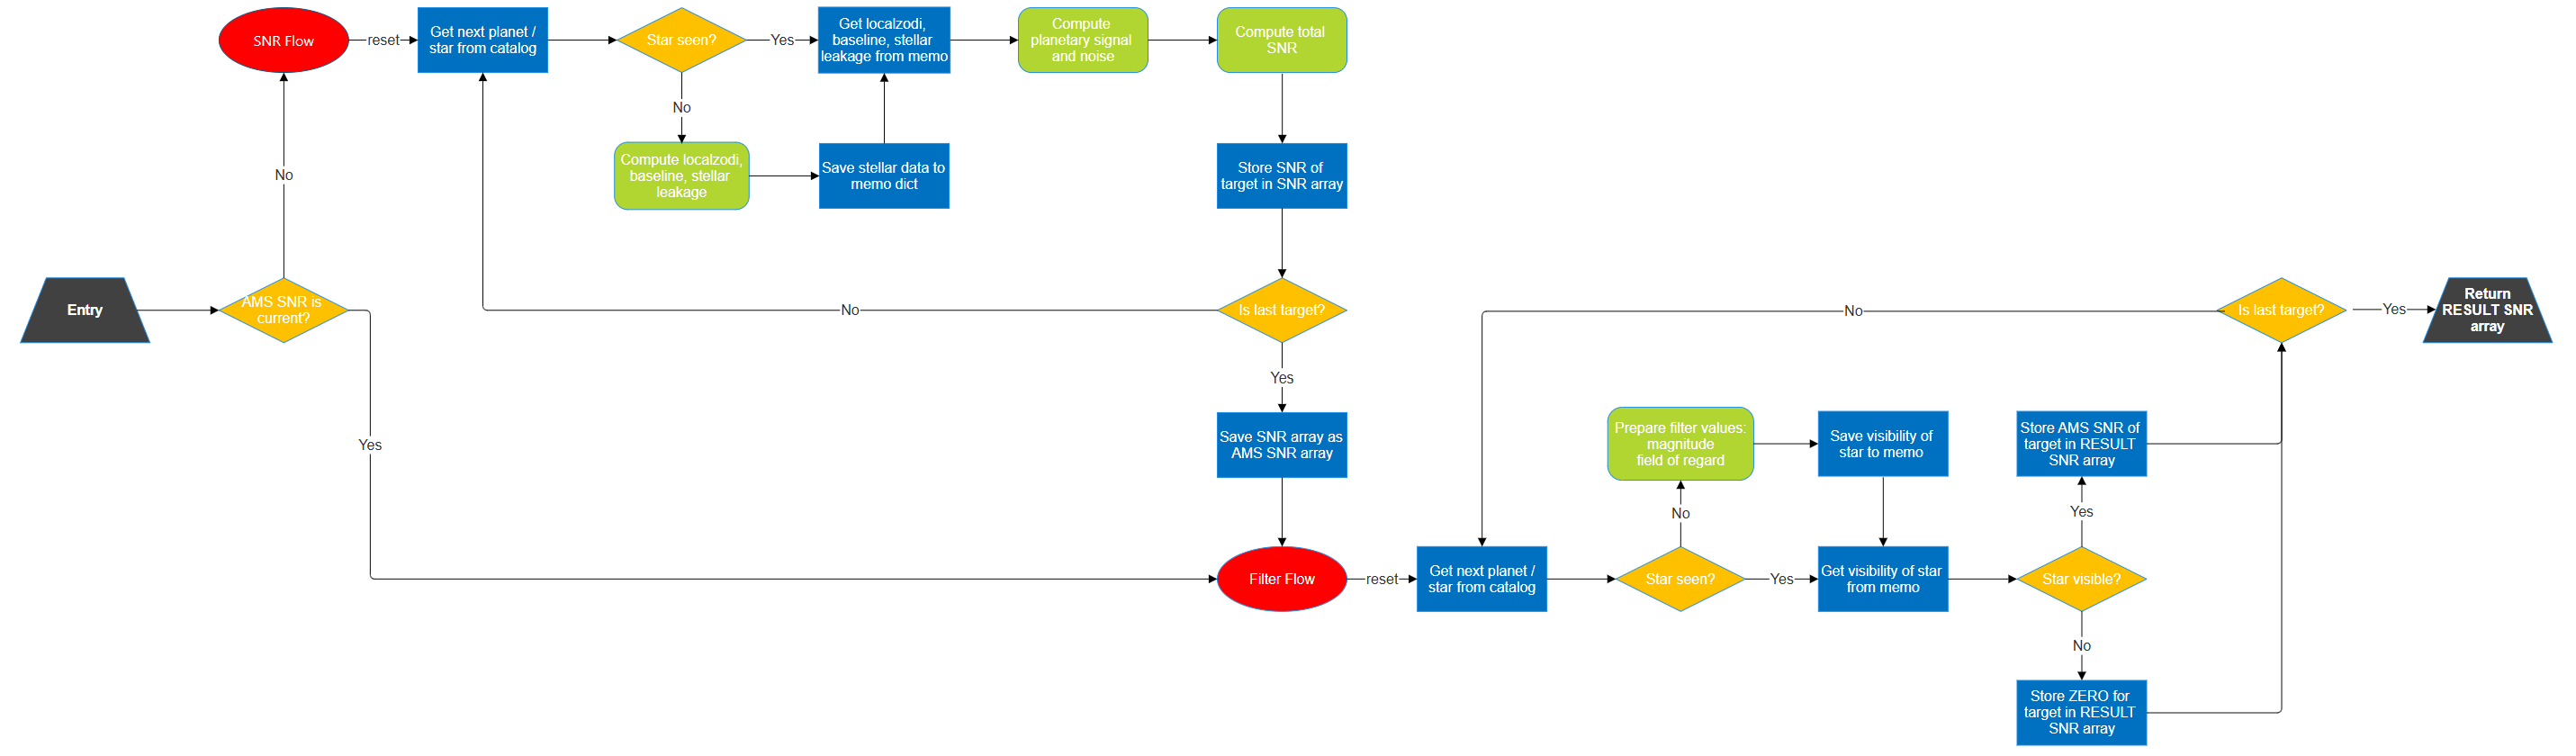
\includegraphics[width=0.95\linewidth]{images/ams_flowchart_simphase.png}
    \caption{AMS simulation phase. Gray trapezoids mark entry or exit, red tiles denote flows, yellow diamonds decisions, green boxes calculations, and blue rectangles memory operations. Physics or budget changes trigger the SNR flow and replace the unfiltered cache. The filter flow always copies that cache and sets targets outside the magnitude or field-of-regard limits to zero; it never destroys unfiltered values.}
    \label{fig: simphase flowchart}
\end{figure}
\end{landscape}
\clearpage

\subsubsection{The Distribution Phase}
We now have a full set of filtered SNRs for every target in the input planet catalog. The only remaining step is to use LIFEsim to distribute the available observation time across the targets and then find the required mission time.

The distribution rests on photon-limited SNR accumulation as the square root of integration time. The SNR flow yields $\text{SNR}_{1\text{h}}$ for each target, so
\begin{align} \label{eq: integration time}
    t_\mathrm{int}(q) = \left(\frac{q}{\text{SNR}_{1\text{h}}}\right)^2\quad\text{[h]}
\end{align}
for a fresh integration to requested bulk SNR $q$. The implemented follow-up calculation does not subtract SNR already accumulated during detection. For a selected planet, with slew time $t_\mathrm{slew}$, it charges
\begin{align}
t_\mathrm{orbit}&=(n_\mathrm{orbits}-1)
\left[t_\mathrm{int}(7)+t_\mathrm{slew}\right],\\
t_\mathrm{char}&=t_\mathrm{int}(44.1)+t_\mathrm{slew}.
\end{align}
This convention treats the four follow-up orbit epochs and the characterization as separate observations. It is intentionally reported as implemented; alternative reuse of detection photons would reduce the follow-up cost.

The complete scheduler is:
\begin{enumerate}
    \item Optimize one common detection sequence over all 100 synthetic universes.
    \item Stop when the inherited strict completion checks report more than 50 qualifying detections in more than 90\% of universes. With 100 universes, this means at least 51 planets in at least 91 universes.
    \item Assign the resulting shared detection-campaign time to every represented universe.
    \item In each universe, retain eligible planets that were detected, rank them by their one-hour SNR at maximum separation, and select the best 50.
    \item Add four orbit follow-ups and one characterization observation per selected planet using the equations above.
    \item Return the 90th percentile of the resulting per-universe total times.
\end{enumerate}

The AMS is consequently a perfect-information ensemble yield model, not an adaptive discovery scheduler. In experiment-limited mode, the configured 0.8 observing efficiency neither caps nor rescales the returned time. Here ``completion of Experiment~1'' always inherits the strict implementation above: at least 51 detections in at least 91 universes, with empty universes omitted from the time sheet. The strict inequalities tend to raise mission time, whereas omission can bias the reported distribution low. Their net effect is not known from the retained outputs.

Two consequences follow for how every time reported in this thesis should be read. First, the returned quantity is the time the scheduler charges: the sum of on-source integration and slew, accumulated over the shared detection campaign, the four orbit follow-ups, and the characterization observation. It is not a calendar duration, because no duty cycle, downlink, calibration, or safe-mode overhead is applied to it. Second, the observing efficiency of 0.8 configured in Table \ref{tab: study assumptions} would, if applied as a duty cycle, map a charged time $T$ to an elapsed duration $T/0.8$; the 5.5-year target used throughout would then correspond to roughly 6.9 years of elapsed mission. Every target, contour, and budget amplitude reported here is stated in charged time, so comparisons among them are internally consistent. They should not be read directly against a mission calendar, and the allowances in Section \ref{sec: tse} are correspondingly optimistic if the reader interprets the target as elapsed time.

The returned percentile is fixed at 90\%. If 100 universe times are retained, a distribution-free binomial calculation gives approximately 95.6\% coverage for the population 90th percentile between the 84th and 96th order statistics. Fewer retained universes require different ranks. The saved final products contain contour endpoints but not every per-universe time vector, so this rank interval cannot be converted into a numerical uncertainty in years or budget amplitude after the fact. Future production runs should retain those vectors and report a corresponding interval alongside every result.

\subsubsection{Validation of the SNR Flow}
The physics and numerical rewrite were checked at several distinct boundaries; Table \ref{tab: validation matrix} states what each check can and cannot establish.

\begin{table}[H]
\centering
\begin{tabular}{@{}p{0.27\linewidth}p{0.27\linewidth}p{0.31\linewidth}@{}}
\toprule
Comparison & Result & Interpretation \\
\midrule
Shared-route SNR comparison (two thousand sampled targets) & Maximum relative difference $4.2\times10^{-16}$ & Confirms wiring and vectorization against shared source modules \\
8-point versus 64-point inverse-wavelength quadrature, $R=5,10,20,50$ & Approximately machine precision for sampled stellar and exozodiacal terms & Establishes convergence of within-bin integration for the retained smooth spectra \\
Analytic azimuthal response versus $2\times10^6$ angle samples, orders 2, 4, 6 & Relative agreement near $10^{-16}$ & Checks the general even-order Bessel reduction \\
Uniform-disk average versus dense two-dimensional grid & Agreement at approximately $10^{-5}$ & Residual is consistent with reference-grid discretization \\
Order-four stellar and local-zodiacal terms versus image sampling, 15 stars & Below 0.7\% at image size 400 & End-to-end check against an independent spatial discretization \\
Exozodiacal radial quadrature self-convergence, orders 2, 4, 6 & Below $10^{-5}$ & Checks the one-dimensional extended-disk integration \\
Order-four and order-six exozodiacal terms versus image sampling & Up to about 10\% on a few stars & Reference-grid aliasing near the Kennedy inner cutoff, not an order-four error: the same stars and grid deviate by 4.5--5.4\% at order two \\
Exozodiacal radial sampling, 25-star check & Worst case 1--3\% after the log-spaced substitution, against up to 35\% before it & A first uniform-in-radius implementation undersampled the steep profile near the inner cutoff; the defect was found by this check and fixed \\
Invalid odd null order & Explicit error & Prevents applying the even-order derivation outside its domain \\
\bottomrule
\end{tabular}
\caption{Validation matrix for the AMS and analytic source calculation. Agreement with shared code establishes numerical consistency, not independent empirical validation of the astrophysical assumptions.}
\label{tab: validation matrix}
\end{table}

The strongest equality---AMS versus the standard source routine---is deliberately narrow: both routes share underlying physical modules. The spatial comparisons and analytic identities provide more independent numerical checks, but none validate the face-on exozodiacal assumption, the scheduler, or the fourth-order proxy as a realizable instrument.

\chapteropening{Trade Space Reduction}{Reducing an intractable parameter space without discarding the relevant physics} \label{sec: ts reduction}
The raw functional trade space cannot be explored directly. This section therefore reduces it in two steps: first by combining admissible independent random terms at one reference plane, and then by replacing spatial pixel grids with analytic integrals where source symmetry permits. Each reduction retains a stated validation boundary.

\subsection{Condensation of Astrophysical Noise} \label{sec: ts reduction: condensation}
The eight unrestricted modifier functions are too conditional to produce a readable engineering bridge quantity. The first reduction therefore asks which terms can be represented by one equivalent independent random-noise contribution without changing their treatment in the SNR variance.

We reduce the trade space by exploiting the additive background terms in the bin variance. We define a wavelength-dependent instrumental term $N_I(\lambda)$; in bin $i$, $N_{I,i}=N_I(\lambda_i)\,\Delta\lambda_i$ is added alongside the corresponding $B_i$ term.
\begin{align*}
N_B(\lambda) = \sum_{i=1}^{n}N_i(\lambda) + N_I (\lambda).
\end{align*}
As is evident from the blackbody behavior of the background noise sources, we must keep the wavelength dependence to maintain physical relevance. Figure \ref{fig: budget example} illustrates the construction: an imposed $N_I(\lambda)$ is added on top of the astrophysical background, and the shaded area between the two curves is the allowance being solved for.

The reduction is valid when terms map to a defined independent random allowance at the same reference plane; it excludes correlated/systematic terms and is not an allocation to subsystems. This study tests flat and two linear-ramp forms of $N_I$, not arbitrary functions. Increasing the amplitude within one specified family increases mission time; the iso-mission-time boundary then defines its tolerated amplitude.
\begin{figure}[htbp]
\centering
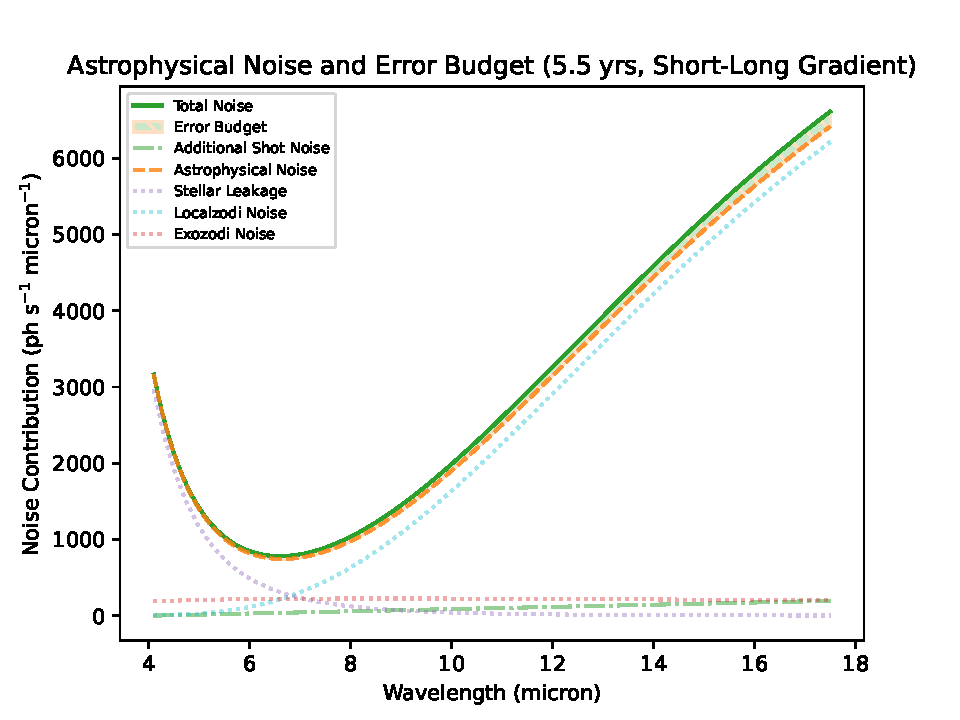
\includegraphics[width=0.8\linewidth]{images/tse/final/no2_hi_long_5p5.pdf}
\caption{Construction of an imposed random-noise budget on top of the astrophysical background. The dashed green line is the imposed $N_I(\lambda)$, here a linear ramp that vanishes at the short-wavelength end of the band and reaches its full amplitude at the long-wavelength end; this is the long-weighted family of Section \ref{sec: tse: budget shape}. The solid green line is the resulting total background including the budget, and the shaded area between the two curves is the allowance itself. All three curves are photon-rate spectral densities referred to the pre-efficiency single-output plane, not variances. The configuration shown is Hab2Max at null order two and the common operating point, with the amplitude set to the largest value compatible with the 5.5-year mission-time target; the same panel recurs among the results as Fig. \ref{fig: tse budget shapes no2}(c).}
\label{fig: budget example}
\end{figure}

\subsection{Analytic Background Evaluation and Spectral Resolution} \label{sec: ts reduction: image spec}
The analytic rewrite of the background evaluation removes the science dependence on image size. Circularly symmetric sources permit an analytic azimuthal and radial reduction of the background integrals: the stellar disk is treated as uniform and circular, local zodiacal light as locally uniform, and exozodiacal light as smooth and face-on. Inclined or asymmetric exozodiacal disks require an angle-resolved treatment and are outside this reduction. Image size now affects visualization and independent cross-checks only, not production science SNR.

The reduction follows from expanding the even power $\sin^{2p}\phi$ into cosines. Azimuthal averaging then uses the standard Bessel integral representation \cite{nistdlmf},
\begin{align}
\frac{1}{2\pi}\int_0^{2\pi}\cos(z\cos\varphi)\,\mathrm{d}\varphi=J_0(z).
\end{align}
For null order $n=2p$, azimuthally averaging one destructive output at angular radius $\vartheta$ gives
\begin{align}
\left\langle T_{2p}\right\rangle_\varphi(\vartheta)
&=
\frac{1}{2}\frac{\binom{2p}{p}}{4^p}
+\sum_{j=1}^{p}(-1)^j\frac{\binom{2p}{p-j}}{4^p}
J_0\left(\frac{2\pi j b\vartheta}{\lambda}\right).
\label{eq: general null average}
\end{align}
For a uniform disk, radial area averaging replaces each $J_0(jx)$ term by $2J_1(jx)/(jx)$, following the standard Bessel derivative identity \cite{nistdlmf}, where $x=2\pi bR/\lambda$ and $R$ is the angular disk radius. The limiting value is one as $jx\rightarrow0$, so the expression is evaluated with its analytic limit near the origin. The Bessel power series then gives the small-star limits
\begin{align}
\left\langle T_2\right\rangle_\mathrm{disk}
&=\frac{x^2}{32}+\mathcal{O}(x^4),\label{eq: leakage small star t2}\\
\left\langle T_4\right\rangle_\mathrm{disk}
&=\frac{x^4}{256}+\mathcal{O}(x^6).
\label{eq: leakage small star}
\end{align}
Taking the ratio of Eqs. \ref{eq: leakage small star t2} and \ref{eq: leakage small star}, the fourth-to-second-order stellar-leakage ratio therefore approaches $x^2/8$. The same general average is used inside one-dimensional radial quadrature for a tapered source or exozodiacal profile. Rotation does not ``average away'' a circular background; rather, circular symmetry makes its integrated response independent of rotation angle \cite{lay2004systematic,dannert2022life2}. Its mean may cancel after chopping, but its photons still set the shot-noise variance.

The local-zodiacal correction arose from a geometric inconsistency in the removed pixel-grid path. That path is inherited LIFEsim code and predates this work; the analytic reformulation did not introduce the defect, it exposed it. The physical field of view is circular, with solid angle proportional to $\pi R_\mathrm{FoV}^2$, but one normalization divided the integrated circular flux by the area $4R_\mathrm{FoV}^2$ of its enclosing square. It therefore suppressed the uniform foreground by $\pi/4$.

The decisive evidence that this is a defect rather than a modelling choice is internal to the inherited code: the untapered branch of the same routine normalized by a circular mask, while the default tapered branch normalized by the square pixel sum, so the two branches disagreed with each other on the same physical configuration. Restoring the circular normalization multiplies the local-zodiacal rate by
\begin{align}
\frac{4}{\pi}=1.2732\ldots
\end{align}
in the uniform limit. That limit is exact only where the product of transmission and field-of-view taper is constant over the domain, which it is not; the ratio measured directly against the old grid is $1.268$. The correction is therefore an increase of approximately 27\%, and the analytic value should not be read as an exact prediction of the measured one. This is a normalization correction, not a new dust model.

Because local-zodiacal shot noise is present for every target, the change propagates nonlinearly through SNR, target ranking, and the 90th-percentile mission time. Comparing the corrected and uncorrected paths over the full \mbox{Hab2Max} catalog gives a median relative SNR shift of about 10.9\%. The scope of that figure should be read carefully: it applies to results computed through the default tapered local-zodiacal path, and the present work does not attempt to propagate it into any previously published LIFE yield number. Doing so would require rerunning those studies and is left to future work.

Transmission and source spectra are integrated within every wavelength bin using an eight-point Gauss--Legendre rule in inverse wavelength $u=1/\lambda$. This coordinate is natural because interferometric phases are proportional to $b/\lambda$ and therefore vary nearly linearly with $u$. Across spectral resolutions 5, 10, 20, and 50 and sampled catalog stars, the stellar-leakage and exozodiacal terms agree with a 64-point reference to approximately machine precision. The adopted resolving power remains $R=\lambda/\Delta\lambda=20$, which produces 31 bins over 4--18.5\,$\upmu$m. Thus spatial image size is no longer a science parameter, while wavelength-bin integration is explicitly converged for the retained binning. Appendix \ref{app: analytic derivation} records the derivation and numerical conventions in greater detail.

\subsection{Restriction of Null Order}
The proxy described in Section \ref{sec: intro: null depth approach} accepts positive even null orders. This thesis evaluates null orders two and four. Order two reproduces the double-Bracewell null envelope; order four is a controlled mathematical proxy using the same four apertures, collecting area, efficiency, baseline ratio, and per-target baseline prescription. No aperture-count or hardware-feasibility claim follows from the fourth-order calculation.

\chapteropening{Trade Space Exploration}{From the reduced parameter space to an iso-mission-time random-noise allowance} \label{sec: tse}
With the trade space reduced, we now invert the AMS mapping. All results use the analytic background model of Section \ref{sec: ts reduction: image spec} and a deliberately conservative common operating point unless a plotted axis varies it. The working LIFE field-of-regard reference is $90^\circ$; $65^\circ$ is substantially more restrictive but still permits acceptable mission times. Current project estimates place the K-band limiting magnitude near 8; magnitude 7 is a pessimistic lower bound, and the completed scans show little remaining sensitivity near that value. A 10\,h slew is the inherited baseline \cite{dannert2025thesis}; 12\,h adds an intentionally simple 20\% margin, while longer slews rapidly remove feasible budget space. The choices are therefore conservative comparison points, not optimized requirements. Hab2Max is evaluated at study targets of 5.5 and 6\,yr; Hab2Min uses 7.5 and 8\,yr. These targets are chosen, not inherited. The LIFE concept is postulated to run for roughly five years, so a shorter target is the more demanding and therefore the more informative requirement; for each catalog the lower target is the smallest half-year step at which a non-trivial positive allowance still exists at the nominal null order. Below it the zero-budget calculation already exceeds the requested time and no allowance can be reported. The second target adds half a year to expose how steeply the allowance responds to a relaxation of the science schedule. Because the two catalogs reach that feasibility threshold at different times, they are not compared at a common mission time; differences between Hab2Max and Hab2Min in Table \ref{tab: budget shapes} therefore combine the occurrence scenario with the different target, and should not be read as an occurrence effect alone. Appendix \ref{app: reproducibility} records this operating point together with the data provenance, the reproduction of the reported amplitudes, and the statistical interpretation of the sampled percentile.

\subsection{The Iso-Mission-Time Budget}
The \textit{iso-mission-time budget} is the tolerated scalar amplitude of one imposed $N_I(\lambda)$ shape at a stated operating point. It is expressed in ph\,s$^{-1}$\,$\upmu$m$^{-1}$ for the flat case or as a ramp endpoint. ``Below'' applies only to the same imposed shape and reference calculation.

The search starts with an amplitude bracket from 0 to 50,000 ph\,s$^{-1}$\,$\upmu$m$^{-1}$. At every iteration the lower bracket endpoint is admissible and the upper endpoint exceeds the target mission time. An exponential fit through the endpoint evaluations proposes the next amplitude; it accelerates the search but does not define the answer. The new evaluation replaces one endpoint according to its mission time, so the bracket invariant is retained. The search stops when mission time lies within 0.05\,yr of the target or the amplitude bracket is at most 10\,ph\,s$^{-1}$\,$\upmu$m$^{-1}$ wide. Reported amplitudes are therefore search point estimates; Section \ref{sec: app: reproduction} quantifies the resulting uncertainty by rerunning the complete search and recording the mission time each reported amplitude actually delivers. The two alternative stopping rules do not support a universal $\pm5$ amplitude uncertainty: a time-tolerance stop may leave a wider amplitude bracket, whereas a bracket-width stop only bounds the final numerical search interval.

Within a fixed target list, added independent variance can only lower individual SNRs. The full mission-time map also includes discrete rankings and a sampled percentile, so global monotonicity is an empirical property rather than a formal theorem. The completed scans showed nested contours and no folded iso-time branches at the sampled resolution. If the zero-budget calculation already exceeds the requested time, no non-negative allowance exists; the plotted dark region represents this physically infeasible operating point, not a failed numerical search.

\subsection{The Shape of the Error Budget} \label{sec: tse: budget shape}
The first question is how the affordable budget depends on its \textit{distribution} over wavelength. We compare three one-parameter families:
\begin{align}
N_\mathrm{flat}(\lambda)&=A,\\
N_\mathrm{short}(\lambda)&=A\,\frac{18.5\,\upmu\mathrm{m}-\lambda}{14.5\,\upmu\mathrm{m}},\\
N_\mathrm{long}(\lambda)&=A\,\frac{\lambda-4\,\upmu\mathrm{m}}{14.5\,\upmu\mathrm{m}}.
\end{align}
Here $A$ is the reported amplitude. The ramp endpoints are imposed shape parameters, not independently inferred wavelength limits. Figures \ref{fig: tse budget shapes no2} and \ref{fig: tse budget shapes no4} show the Hab2Max 5.5-year solutions.

\begin{figure}[htbp]
    \centering
    \begin{subfigure}{.32\textwidth}
        \centering
        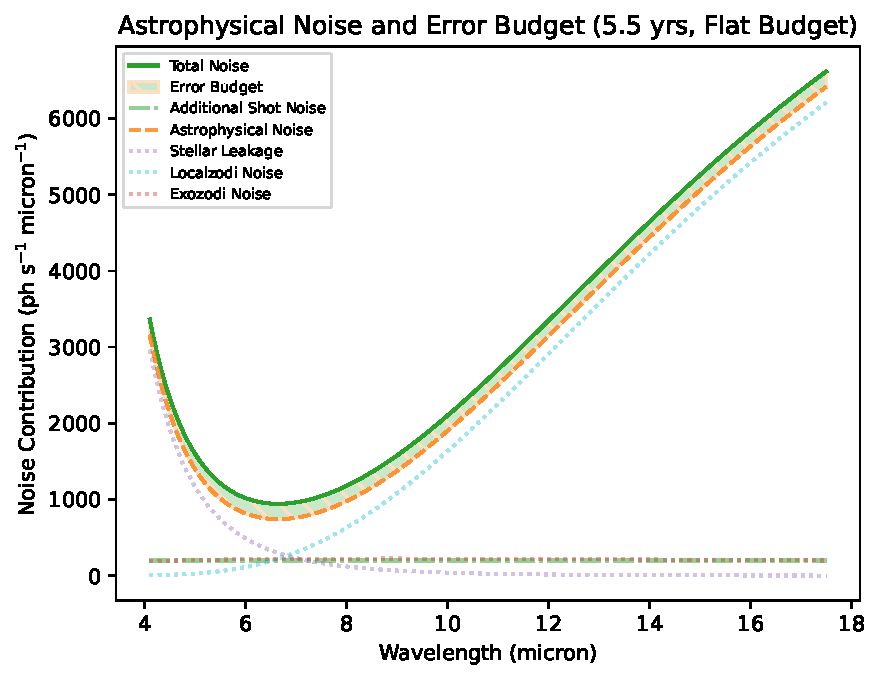
\includegraphics[width=\linewidth]{images/tse/final/no2_hi_flat_5p5.pdf}
        \caption{Flat}
    \end{subfigure}
    \begin{subfigure}{.32\textwidth}
        \centering
        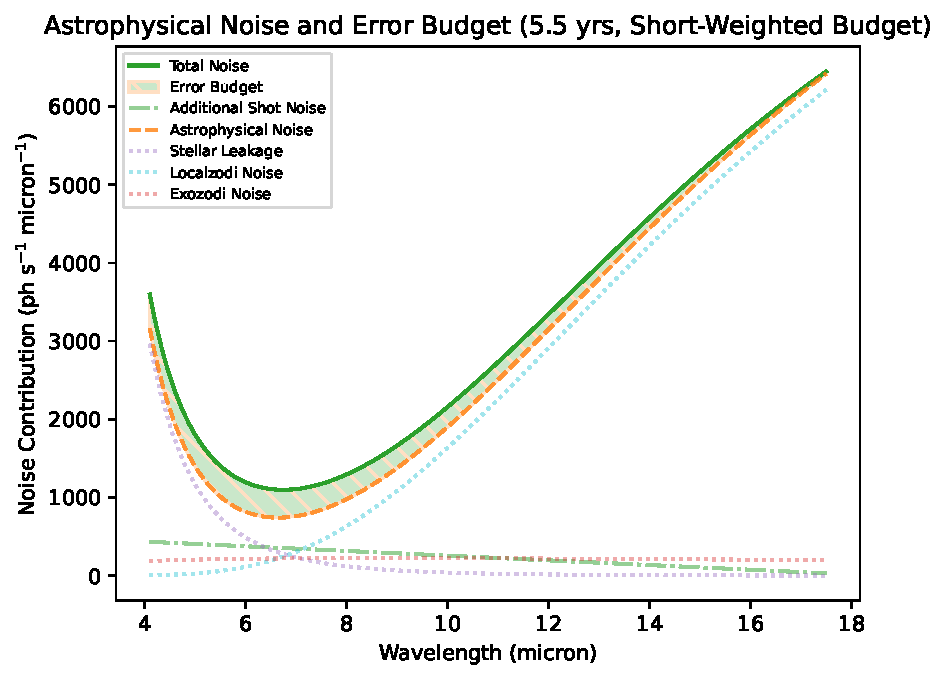
\includegraphics[width=\linewidth]{images/tse/final/no2_hi_short_5p5.pdf}
        \caption{Short-weighted}
    \end{subfigure}
    \begin{subfigure}{.32\textwidth}
        \centering
        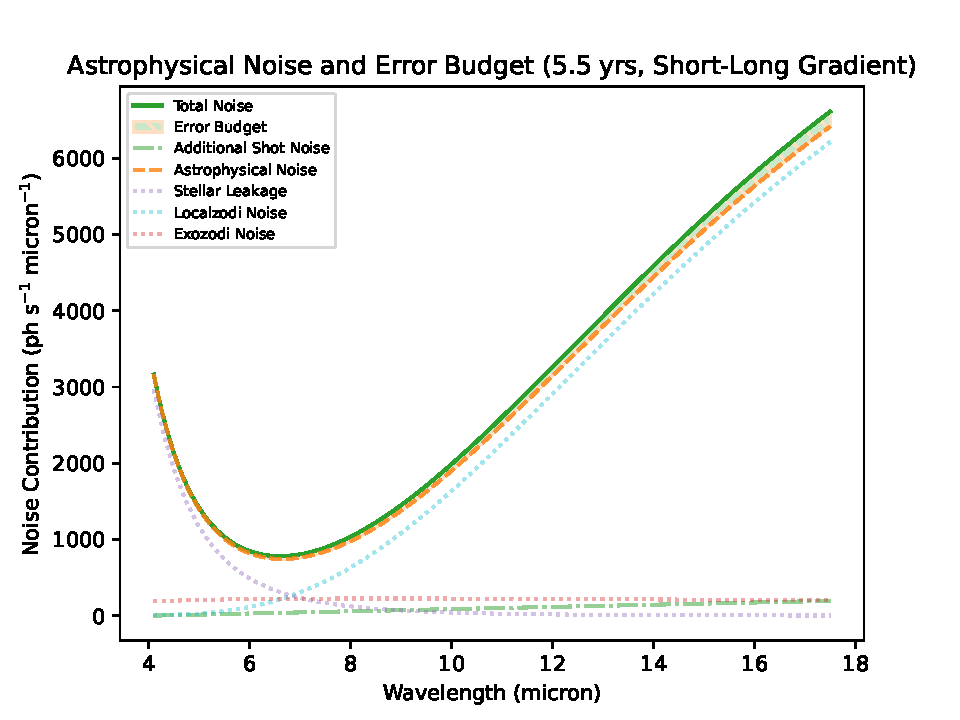
\includegraphics[width=\linewidth]{images/tse/final/no2_hi_long_5p5.pdf}
        \caption{Long-weighted}
    \end{subfigure}
    \caption{Final null-order-two Hab2Max budgets at the common operating point and 5.5-year target. Stellar leakage dominates the short-wave astrophysical background, so the short-weighted ramp admits the largest endpoint.}
    \label{fig: tse budget shapes no2}
\end{figure}

\begin{figure}[htbp]
    \centering
    \begin{subfigure}{.32\textwidth}
        \centering
        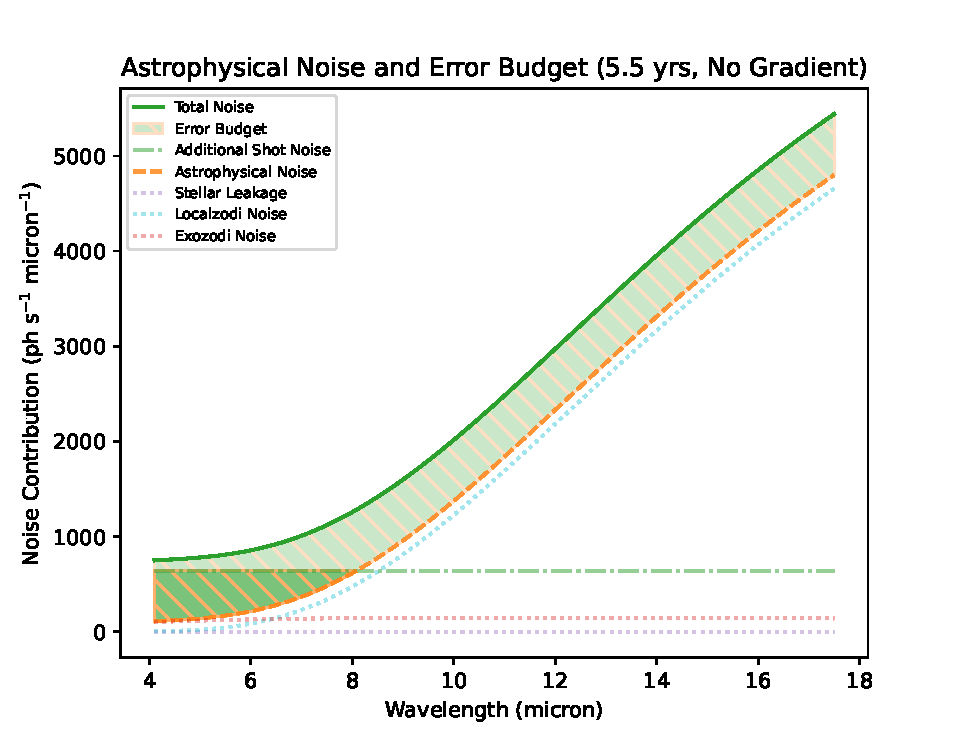
\includegraphics[width=\linewidth]{images/tse/final/no4_hi_flat_5p5.pdf}
        \caption{Flat}
    \end{subfigure}
    \begin{subfigure}{.32\textwidth}
        \centering
        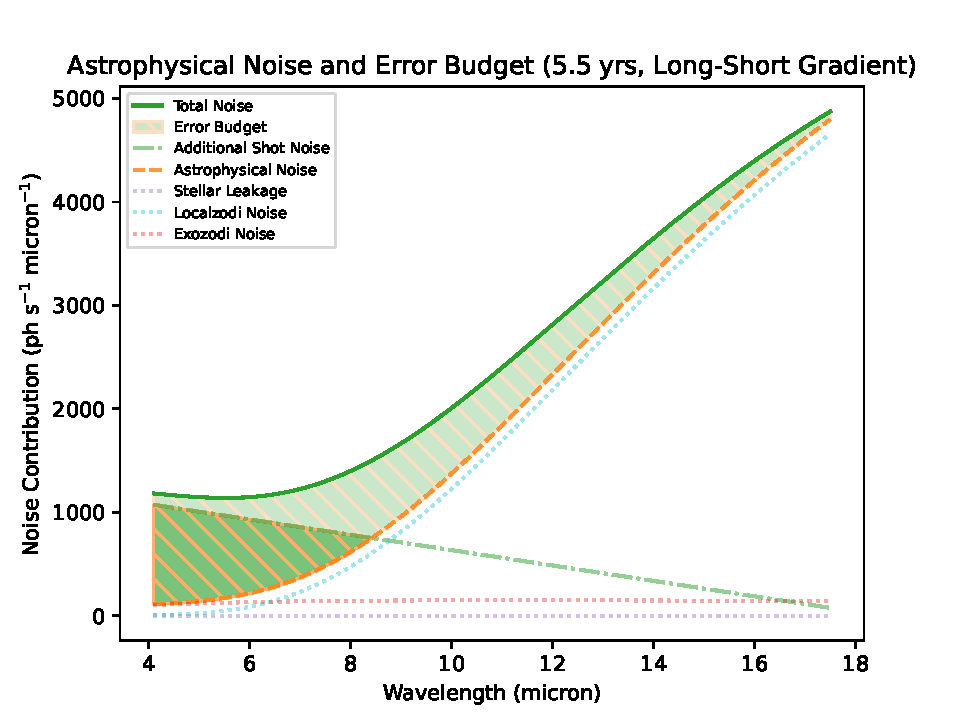
\includegraphics[width=\linewidth]{images/tse/final/no4_hi_short_5p5.pdf}
        \caption{Short-weighted}
    \end{subfigure}
    \begin{subfigure}{.32\textwidth}
        \centering
        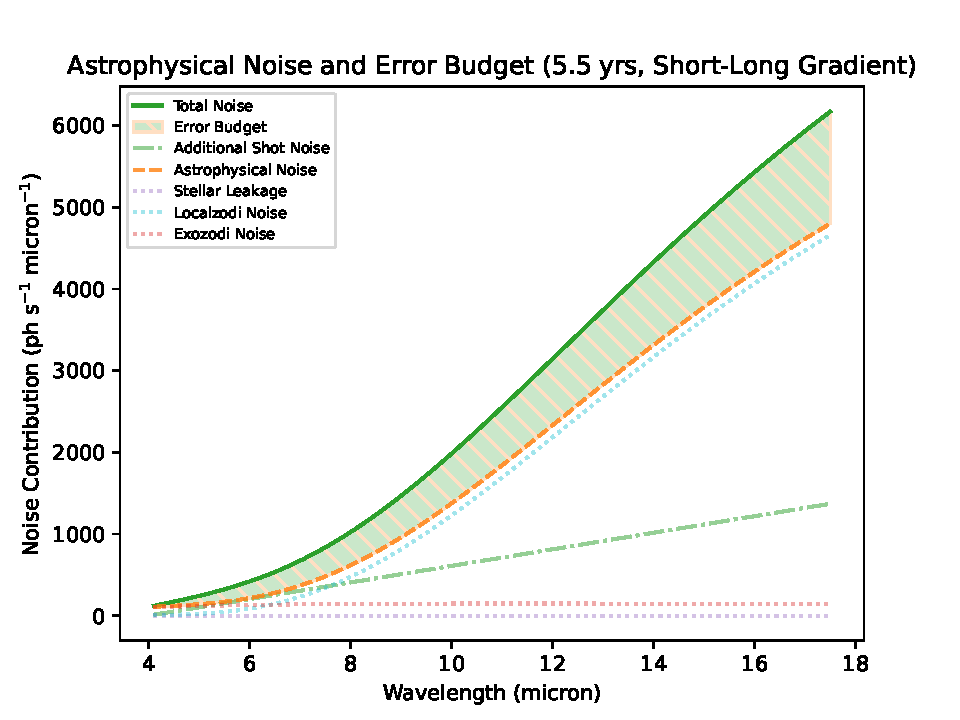
\includegraphics[width=\linewidth]{images/tse/final/no4_hi_long_5p5.pdf}
        \caption{Long-weighted}
    \end{subfigure}
    \caption{Final null-order-four proxy budgets for the same Hab2Max operating point and target as Fig. \ref{fig: tse budget shapes no2}. Geometric stellar leakage is nearly absent. The long-weighted ramp now admits the largest endpoint because the remaining background is dominated by zodiacal emission toward long wavelengths.}
    \label{fig: tse budget shapes no4}
\end{figure}

\begin{table}[htbp]
\centering
\begin{tabular}{@{}llrrrr@{}}
\toprule
Catalog & Mission-time target & Null order & Flat & Short-weighted & Long-weighted \\
        & [yr]      &            & \multicolumn{3}{c}{Amplitude [ph\,s$^{-1}$\,$\upmu$m$^{-1}$]} \\
\midrule
Hab2Max & 5.5 & 2 & 140 & 300  & 210  \\
Hab2Max & 5.5 & 4 & 640 & 1080 & 1470 \\
Hab2Max & 6.0 & 2 & 610 & 1300 & 1090 \\
Hab2Max & 6.0 & 4 & 940 & 1830 & 2240 \\
Hab2Min & 7.5 & 2 & 65  & 200  & 150  \\
Hab2Min & 7.5 & 4 & 590 & 1000 & 1260 \\
Hab2Min & 8.0 & 2 & 460 & 970  & 810  \\
Hab2Min & 8.0 & 4 & 790 & 1460 & 1860 \\
\bottomrule
\end{tabular}
\caption{Final amplitudes at the common operating point. A ramp value is its non-zero imposed endpoint. These endpoint parameters compare sensitivity within the tested families; they are not common integrated-noise measures or engineering-cost rankings.}
\label{tab: budget shapes}
\end{table}

The ordering is consistent across catalogs and both Hab2Max mission-time targets. At null order two, the short-weighted endpoint is largest. At null order four, the long-weighted endpoint is largest. Relaxing the target time also increases the allowance sharply: for example, the Hab2Max flat budget grows from 140 to 610 at order two and from 650 to 940 at order four when the target changes from 5.5 to 6\,yr. For Hab2Min, the corresponding flat allowances rise from 65 to 460 and from 590 to 790 when the target changes from 7.5 to 8\,yr.

A ramp endpoint and a flat amplitude are not directly comparable quantities, so it is worth checking that the reversal is not an artifact of the chosen reporting convention. A ramp rising linearly from zero to $A$ across the band has mean $A/2$, so a flat budget of $A/2$ adds the same band-integrated noise; the integral-neutral ramp endpoint is therefore twice the flat amplitude in the same row. Measured against that reference, the short-weighted endpoint exceeds the neutral value at null order two in all four rows, and the long-weighted endpoint exceeds it at null order four in all four rows. The reversal therefore holds under equal integrated added noise, not only under equal endpoints.

The strong response to a half-year relaxation is not evidence of linear sensitivity. These target times lie near a steep part of the completion curve, where a small SNR loss can move marginal planets below the selected set and where the 90th-percentile universe can change identity. The budget endpoints should therefore be interpolated only through a fresh AMS inversion, not by scaling the values in Table \ref{tab: budget shapes}.

The two-dimensional scans in Fig. \ref{fig: tse linear additive} confirm that the inversion is not an artifact of comparing only the axis endpoints. At order two, equal-mission-time contours extend farther along the short-wavelength-budget axis. At order four, they extend farther along the long-wavelength-budget axis.

\begin{figure}[htbp]
    \centering
    \begin{subfigure}{.49\textwidth}
        \centering
        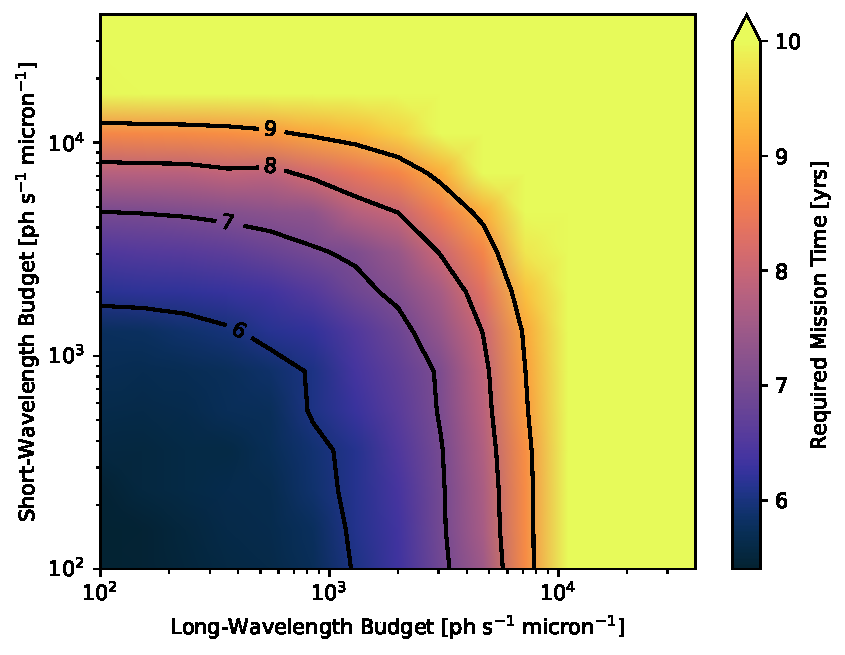
\includegraphics[width=\linewidth]{images/tse/final/no2_hi_linear.pdf}
        \caption{Order 2, Hab2Max}
    \end{subfigure}
    \begin{subfigure}{.49\textwidth}
        \centering
        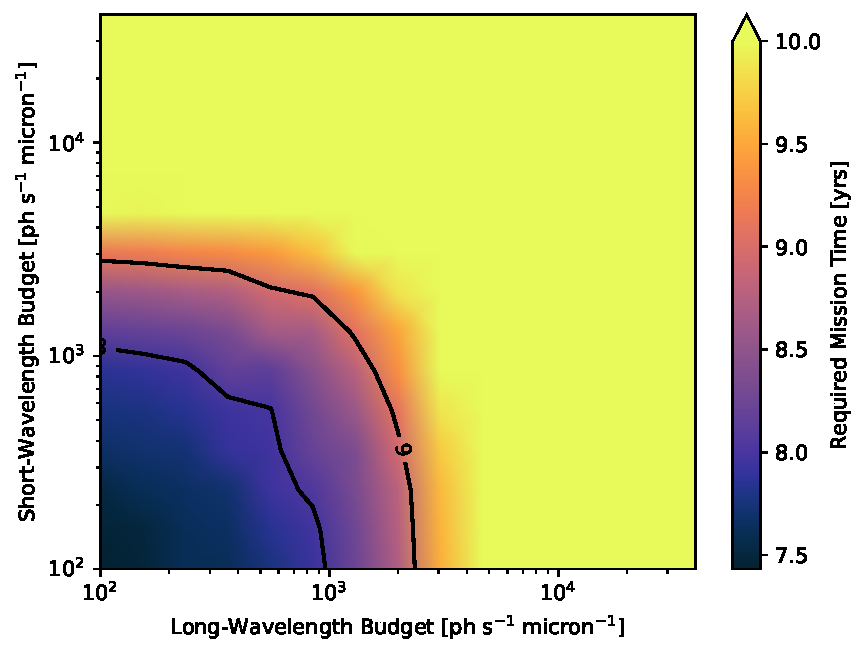
\includegraphics[width=\linewidth]{images/tse/final/no2_lo_linear.pdf}
        \caption{Order 2, Hab2Min}
    \end{subfigure}
    \begin{subfigure}{.49\textwidth}
        \centering
        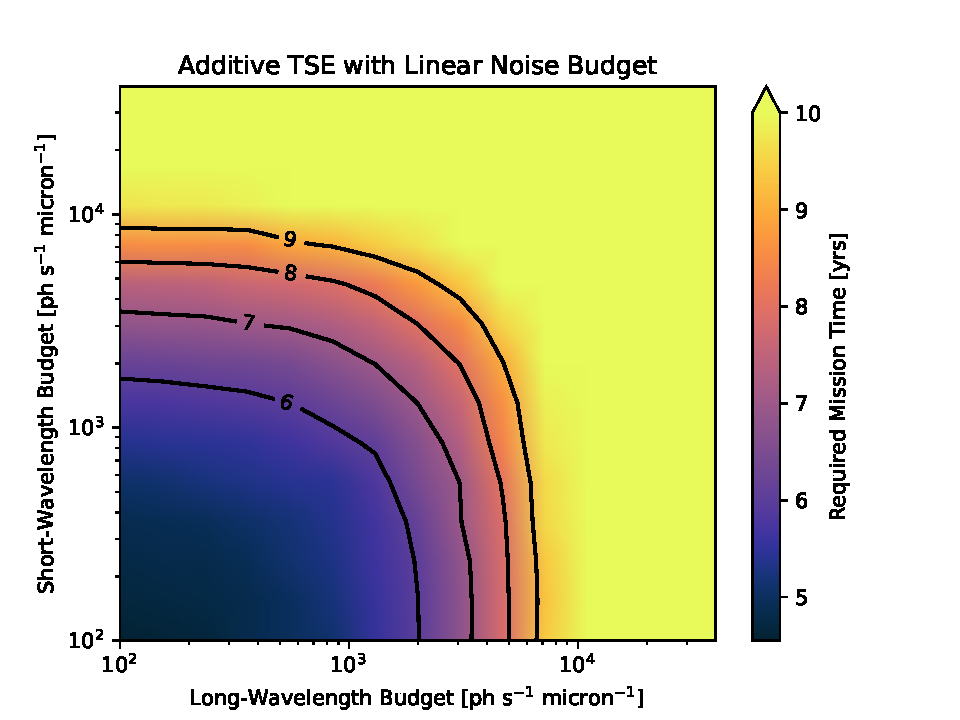
\includegraphics[width=\linewidth]{images/tse/final/no4_hi_linear.pdf}
        \caption{Order 4, Hab2Max}
    \end{subfigure}
    \begin{subfigure}{.49\textwidth}
        \centering
        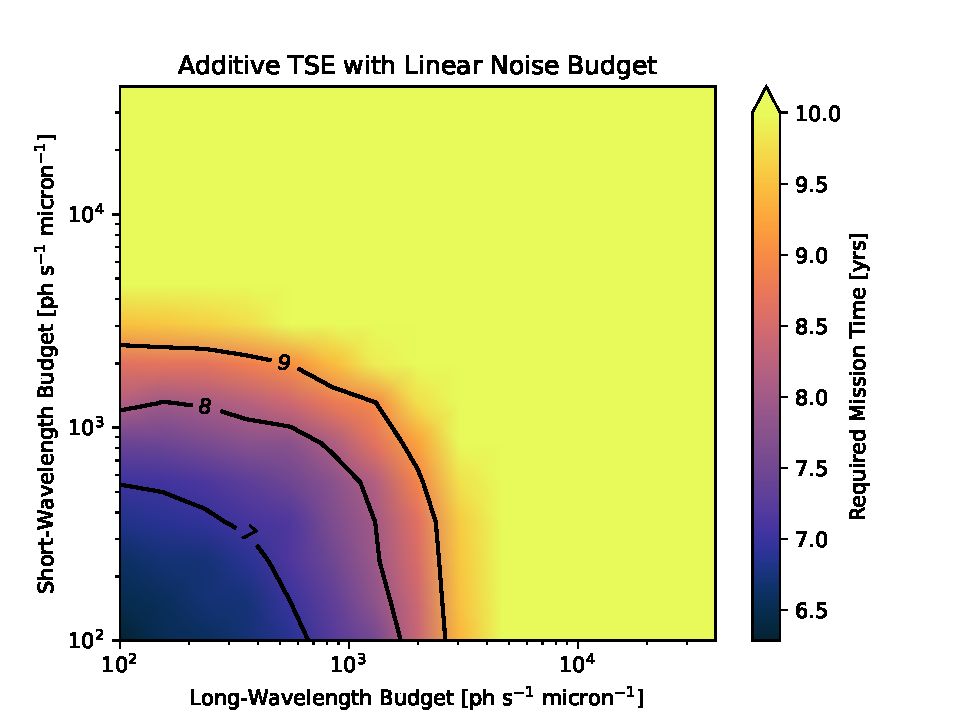
\includegraphics[width=\linewidth]{images/tse/final/no4_lo_linear.pdf}
        \caption{Order 4, Hab2Min}
    \end{subfigure}
    \caption{Required mission time over independent short- and long-wavelength ramp endpoints at magnitude 7, FoR $65^\circ$, and slew 12\,h. Black curves mark integer mission-time contours. The preferred axis reverses between null orders in both catalogs.}
    \label{fig: tse linear additive}
\end{figure}

\subsection{The Random-Noise Error Budget} \label{sec: tse: budget result}
Table \ref{tab: budget shapes} is the numerical answer to the central research question for the tested families and operating points. For any chosen row and shape, amplitudes below the reported value satisfy the corresponding mission-time target under the monotonic-search assumption. The flat family is the most directly comparable scalar allowance. The ramps test where added random variance is least damaging, but their unequal spectral integrals mean that their endpoint amplitudes must not be interpreted as a global cost ranking.

The result also does not provide independent limits at individual wavelengths. For example, the zero at one end of a ramp is imposed by its definition, not inferred from the experiment. Converting these aggregate allowances into an instrument requirement requires a separate allocation model that maps subsystem noise terms to the same reference plane and combines their independent variances.

\subsection{Dependence on the Agnostic Parameters}
The remaining scans use the flat budget and vary two agnostic parameters at a time. They therefore show operating-point dependence of the flat allowance and cannot automatically be transferred to either ramp family.

Figure \ref{fig: tse iso magfor} varies limiting magnitude and field of regard at fixed 12\,h slew time. In all four panels, widening the field of regard has the larger effect because it admits more potential targets. The magnitude dependence largely saturates near the adopted value of 7, especially for Hab2Max: once most high-SNR qualifying stars pass the magnitude cut, admitting still fainter targets adds little to the optimized top-50 sample. Field of regard acts differently because it removes entire sky regions irrespective of target brightness. The fourth-order proxy generally permits a larger flat allowance, but the same qualitative filter dependence remains.

\begin{figure}[htbp]
    \centering
    \begin{subfigure}{.49\textwidth}
        \centering
        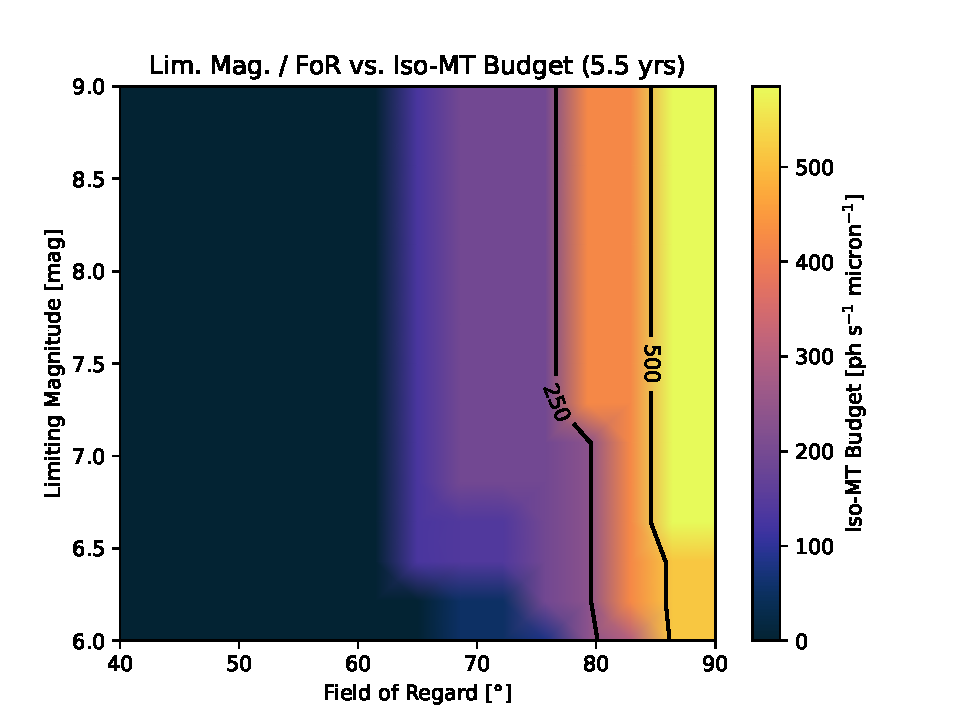
\includegraphics[width=\linewidth]{images/tse/final/no2_hi_magfor_5p5.pdf}
        \caption{Order 2, Hab2Max, 5.5\,yr}
    \end{subfigure}
    \begin{subfigure}{.49\textwidth}
        \centering
        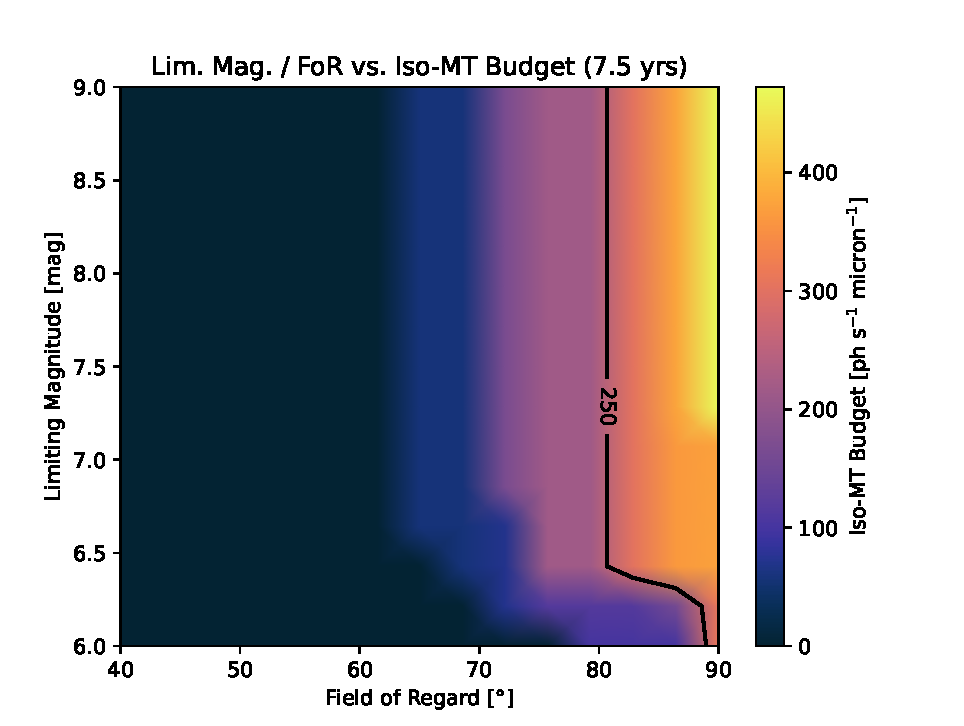
\includegraphics[width=\linewidth]{images/tse/final/no2_lo_magfor_7p5.pdf}
        \caption{Order 2, Hab2Min, 7.5\,yr}
    \end{subfigure}
    \begin{subfigure}{.49\textwidth}
        \centering
        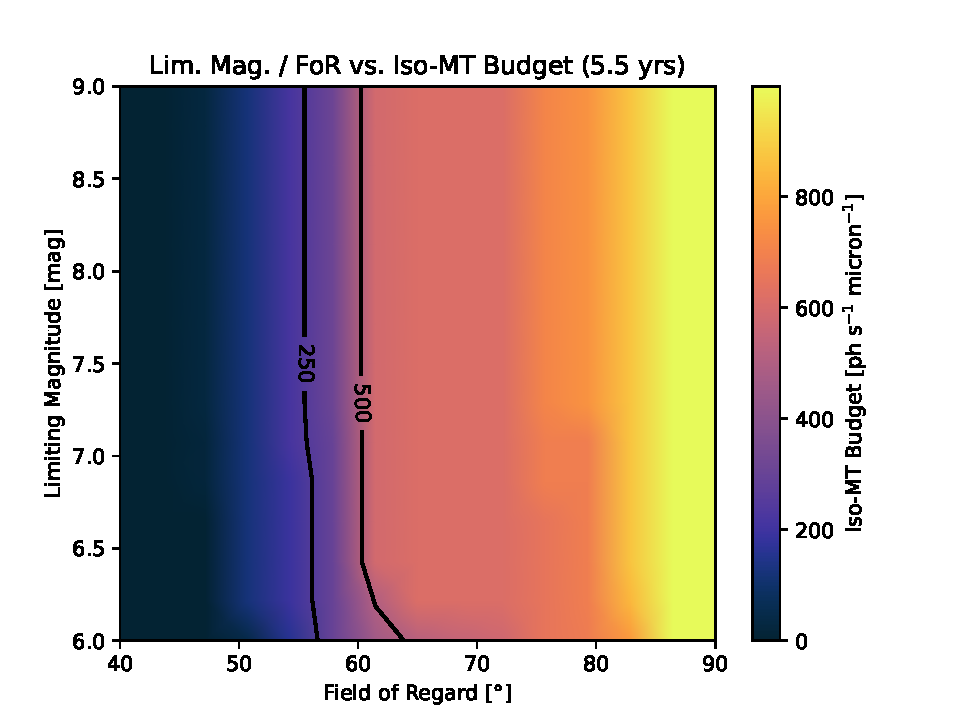
\includegraphics[width=\linewidth]{images/tse/final/no4_hi_magfor_5p5.pdf}
        \caption{Order 4, Hab2Max, 5.5\,yr}
    \end{subfigure}
    \begin{subfigure}{.49\textwidth}
        \centering
        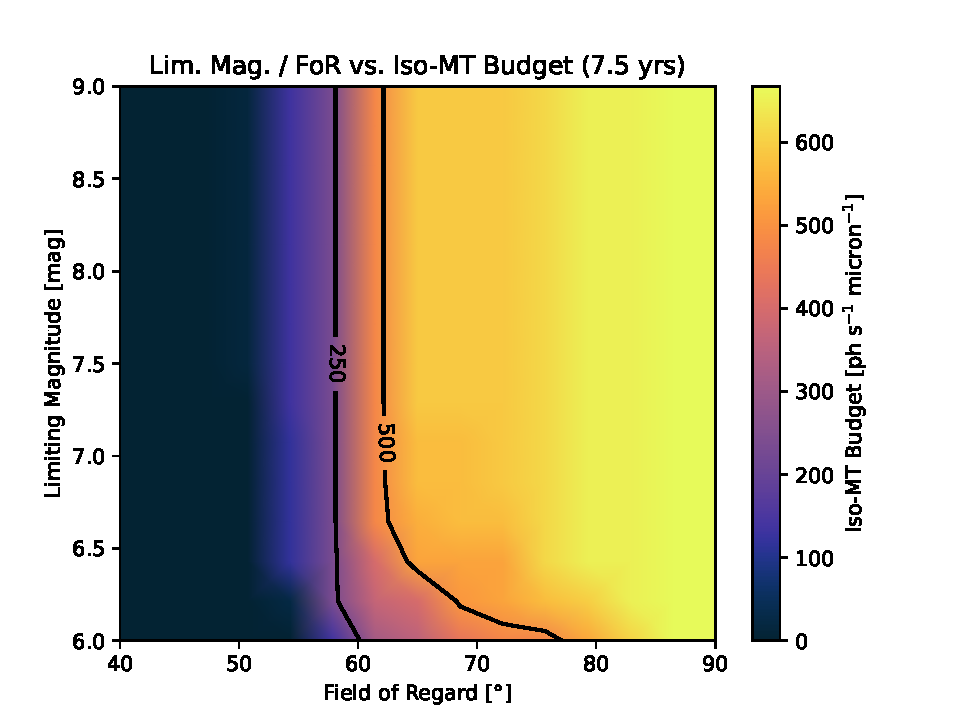
\includegraphics[width=\linewidth]{images/tse/final/no4_lo_magfor_7p5.pdf}
        \caption{Order 4, Hab2Min, 7.5\,yr}
    \end{subfigure}
    \caption{Final iso-mission-time flat-budget scans over limiting magnitude and field of regard, with slew time fixed at 12\,h. Dark regions have no admissible positive budget at the corresponding operating point.}
    \label{fig: tse iso magfor}
\end{figure}

Figure \ref{fig: tse iso slewfor} varies slew time and field of regard at fixed limiting magnitude 7. Longer slews consume time without adding SNR and therefore reduce the admissible budget. The dependence is especially important because each selected planet receives multiple follow-up visits: slew overhead is charged during the shared detection campaign, four additional orbit epochs, and characterization. Wide field of regard and short slew time therefore act together: more targets are available and less overhead is charged for moving between them.

\begin{figure}[htbp]
    \centering
    \begin{subfigure}{.49\textwidth}
        \centering
        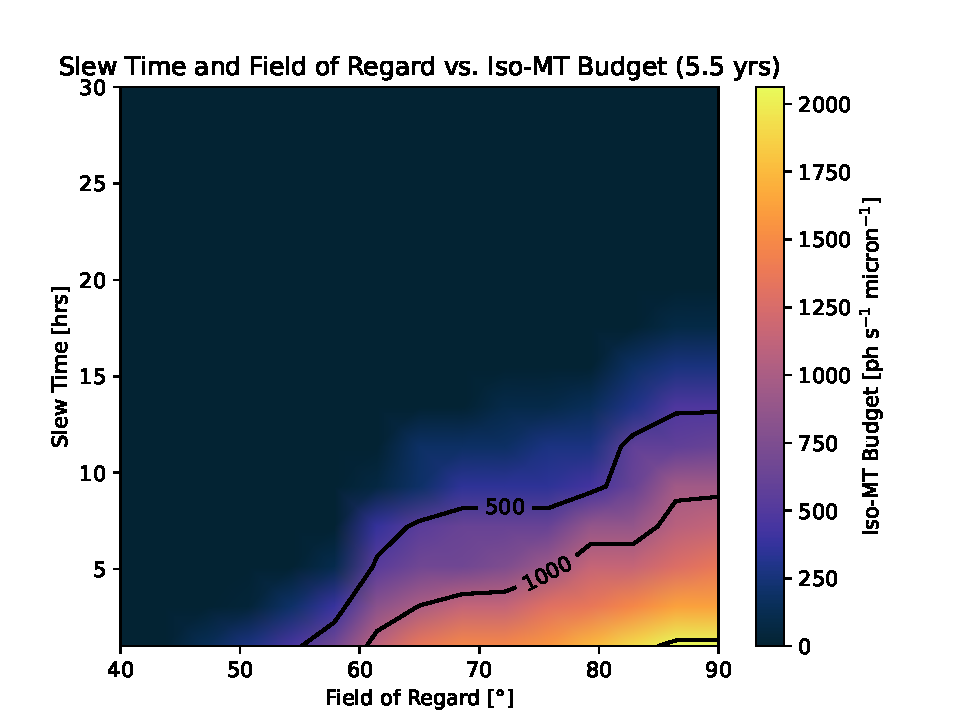
\includegraphics[width=\linewidth]{images/tse/final/no2_hi_slewfor_5p5.pdf}
        \caption{Order 2, Hab2Max, 5.5\,yr}
    \end{subfigure}
    \begin{subfigure}{.49\textwidth}
        \centering
        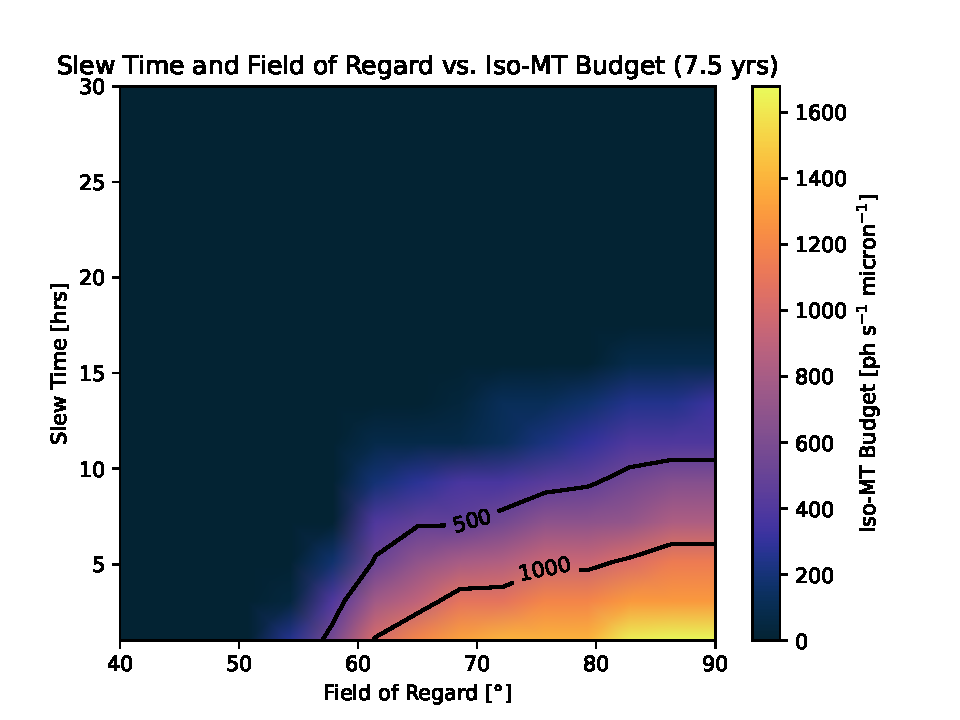
\includegraphics[width=\linewidth]{images/tse/final/no2_lo_slewfor_7p5.pdf}
        \caption{Order 2, Hab2Min, 7.5\,yr}
    \end{subfigure}
    \begin{subfigure}{.49\textwidth}
        \centering
        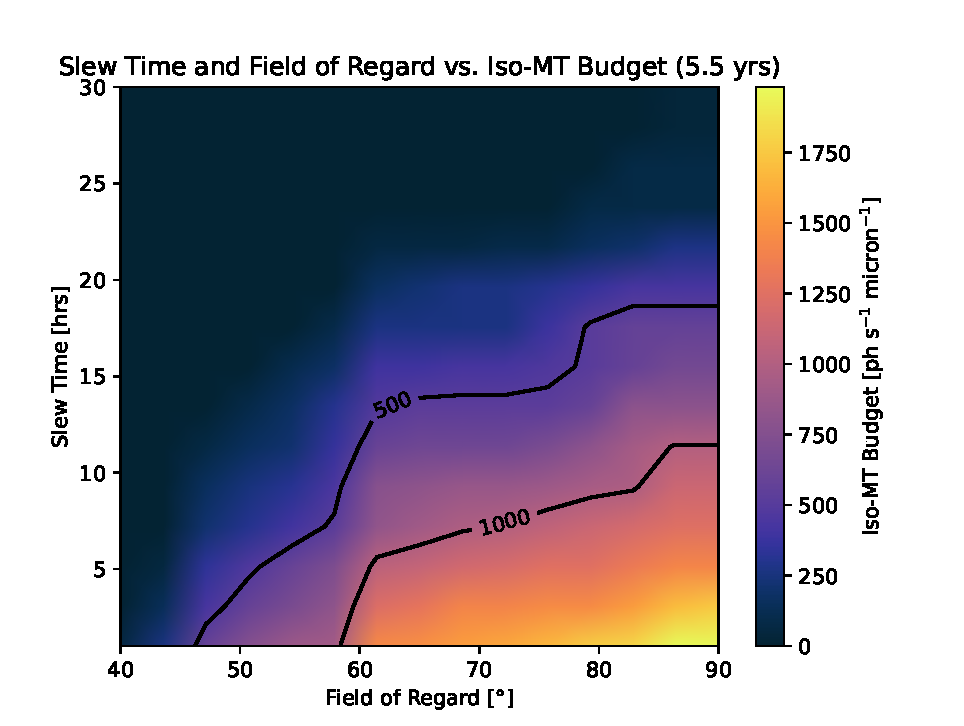
\includegraphics[width=\linewidth]{images/tse/final/no4_hi_slewfor_5p5.pdf}
        \caption{Order 4, Hab2Max, 5.5\,yr}
    \end{subfigure}
    \begin{subfigure}{.49\textwidth}
        \centering
        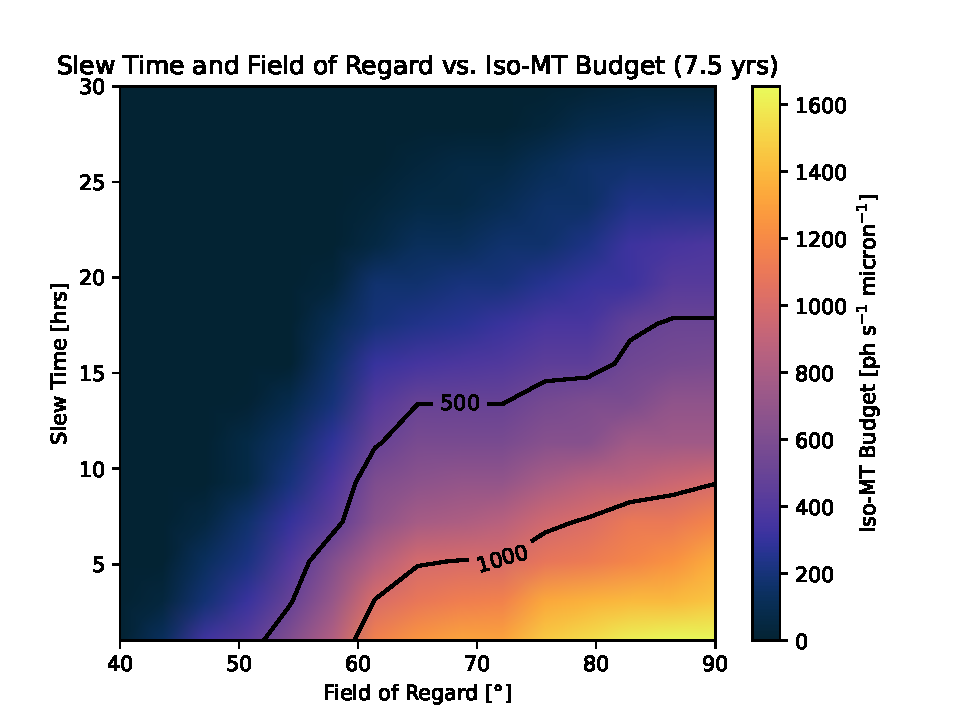
\includegraphics[width=\linewidth]{images/tse/final/no4_lo_slewfor_7p5.pdf}
        \caption{Order 4, Hab2Min, 7.5\,yr}
    \end{subfigure}
    \caption{Final iso-mission-time flat-budget scans over slew time and field of regard at limiting magnitude 7. Dark regions have no admissible positive budget.}
    \label{fig: tse iso slewfor}
\end{figure}

\begin{figure}[htbp]
    \centering
    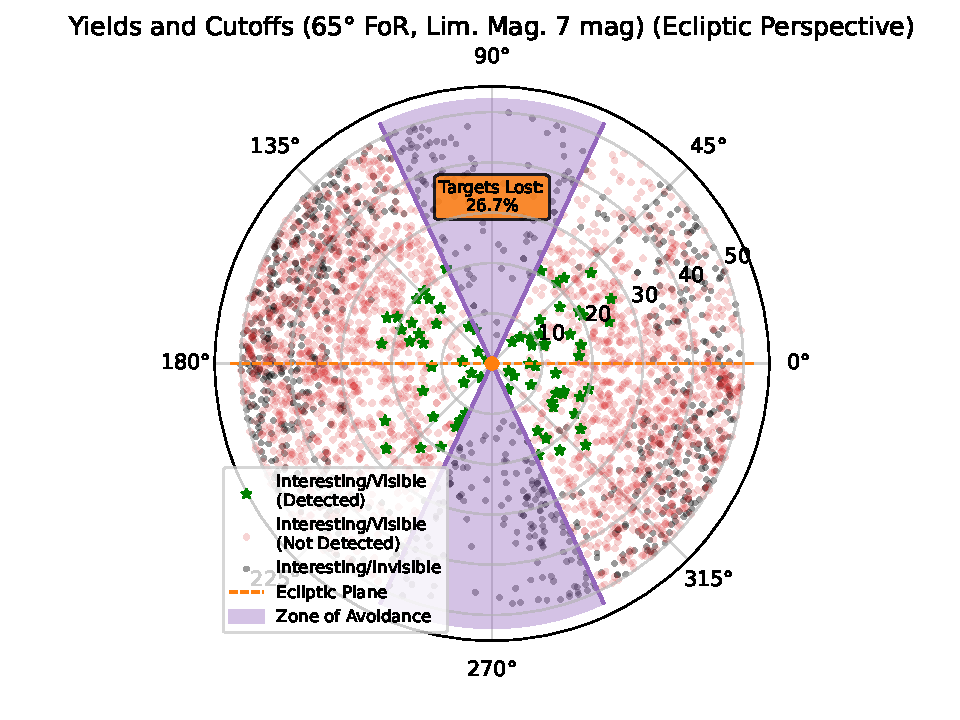
\includegraphics[width=0.7\linewidth]{images/tse/final/no2_hi_yield.pdf}
    \caption{Ecliptic view of the final Hab2Max selection at magnitude 7 and FoR $65^\circ$. Here ``interesting'' denotes Experiment-1-eligible targets. The 26.7\% value is specific to this catalog and selection.}
    \label{fig: tse yield}
\end{figure}

\subsection{Catalog Dependence}
The Hab2Min and Hab2Max calculations show the same qualitative shape ordering and the same null-order inversion. Hab2Min requires longer mission-time targets and generally returns smaller allowances at otherwise matched operating parameters, consistent with its less favorable planet population. Because the adopted mission-time targets differ between catalogs, the numerical difference cannot be attributed to $\eta_\oplus$ alone. Figure \ref{fig: tse yield} illustrates the field-of-regard filter for one Hab2Max selection and is not evidence of catalog independence.

\subsection{Why the Spectral Preference Reverses at Null Order Four} \label{sec: tse: null order}
Suppression of stellar leakage is the leading physical interpretation of the completed order-four comparison. Equations \ref{eq: leakage small star t2} and \ref{eq: leakage small star} together predict a fourth-to-second-order ratio of approximately $x^2/8$. Across the 4505 unique catalog stars, $x=2\pi bR_\star/\lambda$ remains above 0.005 over the modeled band, outside the cancellation-sensitive numerical regime of the direct Bessel sum. At 10\,$\upmu$m the median leakage ratio is about $6.3\times10^{-5}$; at 18.5\,$\upmu$m it is about $1.9\times10^{-5}$. Direct positive quadrature agrees with the analytic order-four response over the complete catalog range.

This suppression removes the high short-wave stellar-noise floor visible in Fig. \ref{fig: tse budget shapes no2}. Added short-wave variance then becomes comparatively expensive. The remaining local- and exo-zodiacal backgrounds dominate toward longer wavelengths, so a larger long-weighted endpoint can be hidden beneath their photon noise. This explanation is consistent with the reversal in Table \ref{tab: budget shapes} and Fig. \ref{fig: tse linear additive}; however, no ablation run isolates leakage suppression from the simultaneous extended-source and planet-throughput changes.

Table \ref{tab: null order synthesis} collects the effects that change between the two orders alongside their consequences for the reported allowance. The result is physical within the proxy but not a standalone architecture prediction. Without throughput normalization, the far-field average of the null envelope changes from $1/4$ at order two to $3/16$ at order four. Local-zodiacal transmission therefore falls by approximately 25\%, and the off-axis planet response also changes. The order-four result consequently combines deeper central suppression with a different throughput distribution while holding all other instrument parameters fixed.

\begin{table}[htbp]
\centering
\begin{tabular}{@{}p{0.28\linewidth}p{0.27\linewidth}p{0.34\linewidth}@{}}
\toprule
Effect & Order-two reference & Order-four proxy consequence \\
\midrule
Near-axis stellar leakage & Leading term $x^2/32$ & Leading term $x^4/256$; median ratio $6.3\times10^{-5}$ at 10\,$\upmu$m \\
Extended-source envelope average & $1/4$ & $3/16$, a 25\% reduction before other weighting \\
Dominant short-wave background & Stellar leakage & Leakage largely removed; added short-wave variance becomes more costly \\
Least damaging tested ramp & Short-weighted & Long-weighted \\
Interpretation & Double-Bracewell reference & Controlled response proxy, not a realizable architecture \\
\bottomrule
\end{tabular}
\caption{Synthesis of the physical and numerical changes behind the null-order inversion.}
\label{tab: null order synthesis}
\end{table}

\subsection{The Throughput Cost of a Deeper Null} \label{sec: tse: throughput}
The null-order proxy holds optical throughput and detector efficiency fixed between orders, as Table \ref{tab: proxy boundary} states. A realizable fourth-order combiner would not: for a fixed four-aperture array, the deep null is available on a smaller fraction of the collected light \cite{guyon2013beam}. The order-four allowances of Table \ref{tab: budget shapes} therefore describe a benefit purchased at a cost the proxy never charges. This section charges it.

The test applies the factor implied by the second- to fourth-order comparison in \cite{guyon2013beam}, halving the total efficiency from $\eta=0.09$ to $0.045$, and repeats the identical endpoint search at the identical operating point. Because $N_I(\lambda)$ is referred to the pre-efficiency plane, scaling the efficiency scales the delivered instrumental noise consistently with the planet signal and the astrophysical background, so the comparison remains at a single reference plane.

The result is unambiguous and negative. At half efficiency, no non-negative allowance exists at any of the four mission-time targets, for either catalog and for any of the three budget families. The reason is not that the budget search fails but that the target is already unreachable before any instrumental noise is added: the zero-budget mission time rises from 4.47 to 7.65\,yr for Hab2Max and from 6.04 to 10.79\,yr for Hab2Min. Both exceed every target in Table \ref{tab: budget shapes}.

Table \ref{tab: throughput sweep} places that single comparison on a curve by evaluating the zero-budget mission time across a range of total efficiencies at both null orders.

\begin{table}[htbp]
\centering
\small
\begin{tabular}{@{}llrrrr@{}}
\toprule
Catalog & Null order & \multicolumn{4}{c}{Zero-budget mission time [yr]} \\
        &            & $\tau=0.15$ & $0.125$ & $0.10$ & $0.075$ \\
\midrule
Hab2Max & 2 & 5.32 & 6.45 & 7.67 & 9.71 \\
Hab2Max & 4 & 4.47 & 5.02 & 6.09 & 7.65 \\
Hab2Min & 2 & 7.41 & 8.60 & 10.40 & 13.27 \\
Hab2Min & 4 & 6.04 & 7.00 & 8.55 & 10.79 \\
\bottomrule
\end{tabular}
\caption{Mission time required with no added instrumental budget, as a function of the optical throughput $\tau$ entering $\eta=\tau\times$ quantum efficiency. The nominal value is $\tau=0.15$; $\tau=0.075$ is the halved-efficiency case used in the ablation. All other parameters are held at the common operating point.}
\label{tab: throughput sweep}
\end{table}

Two features of the table matter. First, mission time grows more slowly than the inverse of throughput. Halving the efficiency multiplies the required time by 1.71 to 1.83 rather than by two, consistently across both catalogs and both orders. In a background-photon-limited regime the integration time alone would scale as $1/\eta$; the shortfall is the slew and overhead component, which is charged per observation and does not scale with efficiency at all. The implied throughput-independent fraction of the mission is 17 to 29\%, largest for the shortest campaigns.

Second, and more consequentially, the throughput penalty is larger than the null-depth benefit at every operating point tested here. Moving from order two to order four at the nominal efficiency saves 0.85\,yr for Hab2Max and 1.37\,yr for Hab2Min; halving the efficiency at fixed null order costs between 3.19 and 5.86\,yr, depending on catalog and order. A fourth-order design that pays the throughput cost implied by \cite{guyon2013beam} is therefore slower than the second-order reference it was meant to improve upon, despite suppressing geometric stellar leakage by three to five orders of magnitude.

Three boundaries limit how far this conclusion can be carried. The baseline prescription constant of Section \ref{sec: methods: AMS} is derived for a second-order double Bracewell and is retained unchanged at order four, so neither arm is baseline-optimal for the deeper null and the measured penalty is an upper bound. The efficiency factor is taken from one specific pair of architectures rather than from a general law relating null order to throughput. And because no target is reachable in the penalized configuration, this test cannot say whether the spectral reversal of Section \ref{sec: tse: null order} survives the penalty; answering that requires repeating the search at mission-time targets beyond 7.65 and 10.79\,yr, which lie outside the range this study set out to examine.

\chapteropening{Discussion}{Interpreting the allowances, the null-order inversion, and their boundaries}
The thesis asks two connected questions: how much aggregate random noise LIFE can tolerate at a chosen mission time, and how that allowance changes when the modeled central null becomes steeper. The completed results answer both within the controlled reference calculation before the methodological and architectural boundaries are considered.

\subsection{The Error Budget and Architecture Comparison}
At the adopted operating point, the nominal second-order null permits flat allowances of 140\,ph\,s$^{-1}$\,$\upmu$m$^{-1}$ for Hab2Max at 5.5\,yr and 65 for Hab2Min at 7.5\,yr. Within the tested ramp families, short-weighted noise is least damaging because it is added where stellar leakage already dominates. This finding is specific to the second-order background hierarchy.

The fourth-order proxy changes that hierarchy. Its corresponding flat allowances rise to 640 and 590, and the long-weighted ramp becomes least damaging. The inversion occurs in both catalogs and in the full two-endpoint contour scans. Its leading interpretation is geometric: the analytic $x^4$ term suppresses stellar leakage and removes much of the short-wave variance floor. The result is robust within the tested proxy, but the absolute improvement cannot be assigned solely to null depth, because the proxy also changes extended-source and planet throughput while leaving the optical efficiency untouched.

Section \ref{sec: tse: throughput} quantifies what that omission is worth, and the answer reverses the engineering reading of the order-four column. Charging the fourth-order configuration the efficiency penalty implied by a realizable four-aperture combiner \cite{guyon2013beam} removes every admissible allowance at every target studied here: the zero-budget mission time alone rises to 7.65\,yr for Hab2Max and 10.79\,yr for Hab2Min. The gain from a deeper null, 0.85 and 1.37\,yr respectively at fixed efficiency, is between three and five times smaller than the cost of halving that efficiency. The order-four allowances should therefore be read as an upper bound on what a deeper null can buy, and the practical conclusion is the opposite of the one the raw comparison suggests: suppressing stellar leakage is worth little if it is paid for in collected photons, and a higher-order architecture is attractive only if it can be built without the accompanying throughput loss. Whether the spectral reversal itself persists under that penalty is not settled here, because no target in the penalized configuration is reachable at all.

\subsection{The Agnostic Approach and the AMS}
The methodological contribution is mechanism-agnostic treatment of an \emph{aggregate} independent random-noise allowance, rather than a subsystem allocation. This common reference-plane quantity allows science completion time to constrain a later engineering allocation without prematurely choosing the physical origin of every random term.

The AMS separates its SNR and filter flows (Section \ref{sec: methods: AMS}). Magnitude, field-of-regard, and slew changes therefore reuse cached unfiltered SNRs, while physical or budget changes trigger recomputation. Host-star memoization further avoids repeated source calculations for planets sharing one star. These boundaries turn the repeated evaluations required by the TSE from an impractical uniform grid into targeted inversions.

\subsection{What the Reductions Buy}
The first reduction combines only independent random terms that can be referred to the same single-output plane as $N_I(\lambda)$ (Section \ref{sec: ts reduction: condensation}). The second replaces spatial-grid evaluation of symmetric backgrounds with exact azimuthal averages and one-dimensional radial quadrature. Together they reduce a formally infinite-dimensional problem to explicit scalar searches, remove image size as a production-science parameter, expose the local-zodiacal normalization error, and provide the analytic null-order scaling used to interpret the result.

\subsection{Limitations}
Table \ref{tab: ranked limitations} ranks the remaining boundaries by their ability to change the numerical allowance or its engineering interpretation.

\begin{table}[htbp]
\centering
\small
\begin{tabular}{@{}p{0.09\linewidth}p{0.22\linewidth}p{0.60\linewidth}@{}}
\toprule
Priority & Limitation & Consequence \\
\midrule
1 & Unnormalized null-order proxy & The order-four comparison combines deeper suppression with changed planet and extended-source throughput; it is not a design prediction. \\
2 & Scheduler boundary behavior & Strict completion tests require at least 51 detections in at least 91 universes, while empty universes are omitted. These choices can bias mission time in opposite directions. \\
3 & Aggregate random-noise model & Correlated instability, calibration bias, and systematic error cannot be allocated from $N_I$ and may impose stricter requirements. \\
4 & Sampling uncertainty & The 100 universes resolve only a sampled 90th percentile. Its 95.6\% distribution-free rank interval spans order statistics 84--96, but saved outputs do not retain the corresponding time amplitudes. \\
5 & Symmetric exozodiacal model & Inclined, clumpy, or asymmetric disks can create rotation-dependent structure absent from the face-on radial reduction. \\
6 & Tested spectral families & Flat and two linear ramps sample three directions in a functional trade space; endpoints are not independent wavelength limits or engineering-cost rankings. \\
\bottomrule
\end{tabular}
\caption{Ranked limitations of the reported error budgets. Priority reflects relevance to the thesis's central numerical and architectural claims, not ease of remediation.}
\label{tab: ranked limitations}
\end{table}

The first limitation sets the strongest boundary on the central comparison. Order four is an impact study of a steeper central null under retained assumptions, not a design prediction. It provides no realizable beam-combination matrix, aperture count, optical-loss model, instability-noise calculation, or control requirement. Likewise, the point estimates inherit both search tolerance and finite-universe rank uncertainty; neither is recoverable as a single symmetric error bar from the retained products.

\subsection{Outlook}
The next scientific step is not another run of the present trade space, but a more physical mapping. A realizable higher-order combiner should replace the $\sin^n$ proxy, including its aperture geometry, normalized throughput, optical losses, and instability terms. The aggregate allowance should then be allocated to concrete subsystems at the same reference plane.

Before another production campaign, the scheduler should use non-strict completion criteria consistent with the stated experiment, retain failed universes explicitly, and save every per-universe component time. This would permit bootstrap or rank-based uncertainty intervals in years and separate detection, orbit, characterization, and slew sensitivities. Extending the analytic framework to inclined or asymmetric exozodiacal disks would remove the next important symmetry assumption. These steps would turn the present defensible impact study into a stronger architecture-level requirement analysis.

\chapteropening{Conclusion}{What the completed simulations establish---and what remains architecture-dependent}
The completed AMS and TSE answer the central research question for every tested budget family and operating point. Under the analytic background model of Section \ref{sec: ts reduction: image spec}, the nominal second-order null permits primary flat allowances of 140\,ph\,s$^{-1}$\,$\upmu$m$^{-1}$ for Hab2Max at 5.5\,yr and 65 for Hab2Min at 7.5\,yr. The order-four proxy raises them to 640 and 590, while the least damaging tested ramp reverses from short-weighted to long-weighted.

The sub-questions close as follows:
\begin{itemize}
    \item The unrestricted AMS trade space contains up to eight free modifier functions and three scalar agnostic parameters and is therefore formally infinite-dimensional. The reported family searches reduce it to one amplitude dimension, four dimensions when all agnostic parameters vary, or five when two ramp endpoints vary independently.
    \item Magnitude, field-of-regard, and slew changes reuse unfiltered SNRs and repeat only filtering and scheduling. Budget, source-physics, or null-order changes require catalog-wide SNR recomputation, although host-shared source terms remain memoized within that pass.
    \item The two reductions must be judged separately, and only one of them is validated here. The \textit{numerical} reduction, analytic integration of the circularly symmetric backgrounds in place of a spatial pixel grid, removes the grid dimension and reproduces the retained source calculation to the precision stated in Table \ref{tab: validation matrix}. The \textit{modelling} reduction, representing all admissible independent random terms by a single aggregate $N_I(\lambda)$ at a common reference plane, removes the unbounded functional dimension and is exact for terms that are genuinely independent and referable to that plane, because independent variances add. What is not tested is how large a fraction of a realistic instrumental noise inventory satisfies that condition. Quantifying the departure for a specific decomposition into subsystem terms is left open, and the sub-question is therefore answered for the numerical reduction and only partially for the modelling one.
    \item The TSE locates maximum flat and linear-ramp amplitudes as iso-mission-time point estimates; Table \ref{tab: budget shapes} reports the complete set, including both catalogs and both mission-time targets.
    \item A fourth-order central null suppresses stellar leakage consistently with the analytic $x^4$ scaling and reverses the spectral preference in both catalogs. This is the leading physical interpretation within the proxy, not an isolated causal proof or a realizable architecture forecast.
\end{itemize}

These allowances do not yet constitute subsystem requirements. They define a validated bridge from scientific yield to an explicit engineering trade space and show which spectral regions most strongly control mission time. That bridge matters because LIFE's promise---new knowledge of nearby terrestrial planets and the possibility of life beyond Earth---depends not only on asking an ambitious question, but on demonstrating that an instrument can answer it within credible limits.

\appendix
\appendixchaptertrue

\chapteropening{Analytic Transmission Derivation}{Derivation of the circularly symmetric transmission and background response} \label{app: analytic derivation}
This appendix records the reduction used by the production source model. It is included to make the fourth-order result independently inspectable without requiring the reader to reconstruct the mathematics from code.

\subsection{Even-Power Reduction}
For a positive even null order $n=2p$, the nulling envelope can be written as a finite cosine series:
\begin{align}
\sin^{2p}x
=\frac{1}{4^p}\left[
\binom{2p}{p}
+2\sum_{j=1}^{p}(-1)^j
\binom{2p}{p-j}\cos(2jx)
\right].
\label{eq: sine power series}
\end{align}
One destructive output contains this envelope multiplied by an imaging factor $\cos^2(\psi\pm\pi/4)$. For an axisymmetric source, the complementary imaging phase contributes one half after full azimuthal integration. Let a sky point at angular radius $\vartheta$ have projected nulling coordinate $\alpha=\vartheta\cos\varphi$. Substituting $x=\pi b\vartheta\cos\varphi/\lambda$ into Eq. \ref{eq: sine power series} and using the NIST Digital Library of Mathematical Functions integral representation \cite{nistdlmf},
\begin{align}
\frac{1}{2\pi}\int_0^{2\pi}
\cos(z\cos\varphi)\,\mathrm{d}\varphi=J_0(z)
\end{align}
gives Eq. \ref{eq: general null average}. The reduction is exact for the proxy response and any circularly symmetric surface-brightness profile. It is not an approximation based on rapid rotation.

For the two orders used in the thesis,
\begin{align}
\left\langle T_2\right\rangle_\varphi
&=\frac14\left[1-J_0\left(\frac{2\pi b\vartheta}{\lambda}\right)\right],\\
\left\langle T_4\right\rangle_\varphi
&=\frac1{16}\left[
3-4J_0\left(\frac{2\pi b\vartheta}{\lambda}\right)
+J_0\left(\frac{4\pi b\vartheta}{\lambda}\right)
\right].
\end{align}
At large phase, the oscillatory Bessel terms approach zero. The corresponding far-field averages are therefore $1/4$ and $3/16$. This is the origin of the throughput caveat in the main text.

\subsection{Uniform-Disk Average and Small-Star Limit}
For a uniform disk of angular radius $R$, area averaging a radial Bessel term gives, using the Bessel derivative identity \cite{nistdlmf},
\begin{align}
\frac{2}{R^2}\int_0^R
\vartheta J_0(a\vartheta)\,\mathrm{d}\vartheta
=\frac{2J_1(aR)}{aR}.
\label{eq: disk bessel average}
\end{align}
The right-hand side is evaluated as one when $aR=0$. With $x=2\pi bR/\lambda$, the disk-averaged responses become
\begin{align}
\left\langle T_2\right\rangle_\mathrm{disk}
&=\frac14\left[1-\frac{2J_1(x)}{x}\right],\\
\left\langle T_4\right\rangle_\mathrm{disk}
&=\frac1{16}\left[
3-\frac{8J_1(x)}{x}+\frac{2J_1(2x)}{2x}
\right].
\end{align}
The second-order result is not new: Eq. \ref{eq: disk bessel average} applied to the double-Bracewell response reproduces the uniform-disk stellar leakage given by Lay \cite{lay2005imaging}. What the derivation above adds is the extension to arbitrary even null order through the general coefficient sum of Eq. \ref{eq: general null average}, and its reuse inside the one-dimensional radial quadrature for tapered and extended sources in Section \ref{sec: ts reduction: image spec}, neither of which follows from the second-order case alone.
Using the standard Bessel power series \cite{nistdlmf}, $J_1(x)=x/2-x^3/16+x^5/384+\mathcal{O}(x^7)$, which yields
\begin{align}
\left\langle T_2\right\rangle_\mathrm{disk}
&=\frac{x^2}{32}-\frac{x^4}{768}+\mathcal{O}(x^6),\\
\left\langle T_4\right\rangle_\mathrm{disk}
&=\frac{x^4}{256}+\mathcal{O}(x^6).
\end{align}
Consequently,
\begin{align}
\frac{\left\langle T_4\right\rangle_\mathrm{disk}}
{\left\langle T_2\right\rangle_\mathrm{disk}}
=\frac{x^2}{8}+\mathcal{O}(x^4).
\end{align}
This scaling predicts the near-disappearance of geometric stellar leakage before any mission scheduling is performed. Direct positive quadrature is retained as a numerical safeguard where subtraction of nearly equal Bessel terms could lose precision.

\subsection{Radial Profiles and Wavelength Bins}
For a circular source with surface brightness $I_\lambda(\vartheta)$, the transmitted spectral photon rate is proportional to
\begin{align}
2\pi\int_0^{R_\mathrm{max}}
I_\lambda(\vartheta)
\left\langle T_n\right\rangle_\varphi(\vartheta)
\vartheta\,\mathrm{d}\vartheta.
\end{align}
This single radial integral replaces a two-dimensional pixel sum. The stellar disk terminates at its angular radius; the exozodiacal calculation uses the adopted smooth radial brightness profile and field-of-view taper. A source lacking circular symmetry cannot be reduced in this way.

For wavelength-bin edges $\lambda_-$ and $\lambda_+$, the calculation changes variables to $u=1/\lambda$:
\begin{align}
\int_{\lambda_-}^{\lambda_+}f(\lambda)\,\mathrm{d}\lambda
=\int_{1/\lambda_+}^{1/\lambda_-}
\frac{f(1/u)}{u^2}\,\mathrm{d}u.
\end{align}
Eight-point Gauss--Legendre quadrature is then applied over the finite $u$ interval. Because the interferometric phase is proportional to $u$, this samples chromatic fringes more uniformly than the same number of points placed directly in wavelength.

\subsection{Local-Zodiacal Solid Angle}
For a locally uniform foreground with spectral radiance $I_\lambda$, the photon rate is proportional to the accepted solid angle. In the small-angle approximation, a circular field with angular radius $R_\mathrm{FoV}$ has
\begin{align}
\Omega_\mathrm{circ}=\pi R_\mathrm{FoV}^2.
\end{align}
The removed grid implementation integrated pixels inside this circle but normalized one path with the enclosing square area $\Omega_\mathrm{square}=4R_\mathrm{FoV}^2$. Its result was therefore low by
\begin{align}
\frac{\Omega_\mathrm{circ}}{\Omega_\mathrm{square}}=\frac{\pi}{4}.
\end{align}
The corrected rate is the former rate multiplied by $4/\pi$. The current analytic calculation uses the circular solid angle directly, consistent with the continuous field-of-view convention in the LIFE source model \cite{dannert2022life2}.

\chapteropening{Reproducibility and Statistical Interpretation}{Operating-point records and interpretation of the sampled mission-time percentile} \label{app: reproducibility}

\subsection{Operating Point and Search Products}
Unless an axis is explicitly varied, every reported contour uses limiting K-band magnitude 7, implemented field of regard $|\beta_\mathrm{ecl}|\leq65^\circ$, and 12\,h slew time. The flat, short-weighted, and long-weighted families are evaluated independently. A ramp amplitude always denotes its non-zero endpoint, and its other endpoint is constrained to zero by definition.

The completed products are sufficient to reproduce the reported contour endpoints and figures from the saved AMS outputs. They are not sufficient to recompute a different population quantile or a confidence interval in years because individual universe times were not retained for every evaluated amplitude. Reproducibility of future studies would improve by storing, for every search evaluation:
\begin{itemize}
    \item the complete per-universe detection, orbit, characterization, and slew times;
    \item the selected target identifiers and one-hour SNRs;
    \item the lower and upper amplitude bracket and the stopping reason;
    \item the exact catalog, source-model, and scheduler configuration;
    \item the proxy null order and whether throughput was normalized.
\end{itemize}

\subsection{Data and Source Provenance}
The reformulation of the astrophysical background evaluation described in Section \ref{sec: ts reduction: image spec} was documented in a standalone technical brief covering its derivation, its validation boundaries, and the local-zodiacal normalization correction, and was reviewed and accepted by the thesis supervisor. The code state carrying that reformulation has since been placed under version control; the source hash below remains the authoritative identifier for the production campaign, because the working tree was not clean when those calculations were run.

Table \ref{tab: provenance hashes} records the exact local inputs and result closure used for the final thesis. SHA-256 hashes make later identity checks possible even though no immutable public archive or complete environment lock was created during the production campaign. The source hash covers the production-code closure used by the completed calculations; the result hash covers the 52 files in the complete \texttt{TSE Linear} result tree from which the thesis figures and values were taken.

\begin{table}[htbp]
\centering
\small
\begin{tabular}{@{}p{0.24\linewidth}p{0.25\linewidth}p{0.43\linewidth}@{}}
\toprule
Artifact & Size or count & SHA-256 \\
\midrule
Hab2Min catalog & 126\,552\,381 bytes & \nolinkurl{8a43af800ed5bb7540a0656506057dbb4f9dabc6be553fcf510f767ccd751aee} \\
Hab2Max catalog & 190\,077\,716 bytes & \nolinkurl{c372e4f665856ceb2ea7dc4c0e059b8447a119586e75e74e98001c3425da9799} \\
Production source closure & commit \texttt{2fd5142}, plus recorded working tree & \nolinkurl{00751d7dca7c095819401bd95c8ccfb64a5778ccd39469c9935eb29673b12b90} \\
Complete final result tree & 52 files; 1\,895\,071 bytes & \nolinkurl{61889403be458b5ac65bc7c63bde4eebf260a6251d5ed4bca3e0c2dd1d3181cc} \\
Validation scripts & recorded script closure & \nolinkurl{040dd0bca26ba14c17a2b8cbed2745e0fa444d0c8956c851e388e442fc1897b1} \\
\bottomrule
\end{tabular}
\caption{Identity record for the catalogs, production source, completed result tree, and validation scripts used in this work. The repository was not clean at production time; the source-tree hash, rather than the commit identifier alone, defines the recorded code state.}
\label{tab: provenance hashes}
\end{table}

The retained \texttt{TSE Linear} products contain rendered PDFs and text summaries, not raw per-evaluation grids, logs, or per-universe time vectors. The order-four Hab2Min 8-year ramp values were recovered from the complete vector result PDFs and cross-checked by reproducing the corresponding 7.5-year values before rounding to the precision used in Table \ref{tab: budget shapes}. Consequently, the final figures and tabulated endpoints are traceable, but the production campaign cannot be rerun bit-for-bit from this record alone. A practical future release should archive the catalogs or their immutable source identifiers, the full code closure, an environment lock, the run matrix, raw grids, scheduler logs, and per-universe outputs.

\subsection{Independent Reproduction of the Final Amplitudes} \label{sec: app: reproduction}
The amplitudes of Table \ref{tab: budget shapes} were produced during a campaign in which the working tree was not clean, and the raw per-evaluation products were not retained. To establish that they are nevertheless reproducible, the complete endpoint search was rerun from a committed code state at the identical operating point, using a single dedicated script whose output is the machine-written table below. The rerun additionally records the mission time that each reported amplitude actually delivers, which the original campaign did not retain.

That last quantity matters for interpretation. The search stops once the evaluated mission time lies within 0.05\,yr of the target, and it returns its last accepted amplitude, so a reported value belongs to the achieved time rather than to the nominal target. The residuals of the rerun span $-0.044$ to $+0.034$\,yr, within the stopping tolerance by construction. Converting a residual into an amplitude uncertainty requires the local slope of amplitude against mission time, which the secant between each catalog's two targets estimates as roughly $6\times10^{2}$ to $1.5\times10^{3}$\,ph\,s$^{-1}$\,$\upmu$m$^{-1}$ per year. The stopping tolerance therefore corresponds to an amplitude uncertainty of order 20 to 80\,ph\,s$^{-1}$\,$\upmu$m$^{-1}$, depending on the row. Because the response is not linear in mission time, these figures indicate the scale of the search uncertainty rather than a calibrated interval, and they are the reason no reported amplitude should be read to better than its leading two digits.

Of the twenty-four amplitudes in Table \ref{tab: budget shapes}, twenty reproduce to the precision reported there and four differ by a single rounding step: the Hab2Max six-year order-four short-weighted value, the Hab2Min seven-and-a-half-year flat values at both orders, and the Hab2Min seven-and-a-half-year order-two long-weighted value. All four differences are smaller than the search uncertainty estimated above, and no difference exceeds one step. The Hab2Min eight-year rows reproduce throughout; those values had previously been recovered from vector plots rather than from retained numerical output, and are now re-derived directly from the code.

The reproduction also exposes an inconsistency in the reporting convention rather than in the calculation. Table \ref{tab: budget shapes} rounds most amplitudes to the nearest ten, but the smallest entry is given as 65, which is neither the nearest ten nor two significant figures of the reproduced 62.2. Small amplitudes are where the fixed time tolerance translates into the largest relative uncertainty, so they are also where a rounding convention matters least and misleads most; the values in Table \ref{tab: reproduction} should be preferred where the two disagree.

\begin{table}[htbp]
\centering
\small
\begin{tabular}{@{}llrrrl@{}}
\toprule
Catalog & Target & Flat & Short-weighted & Long-weighted & Achieved time \\
        & [yr] & \multicolumn{3}{c}{Amplitude [ph\,s$^{-1}$\,$\upmu$m$^{-1}$]} & [yr] \\
\midrule
\multicolumn{6}{@{}l}{\textit{Null order two}} \\
Hab2Max & 5.5 & 142.4 & 298.3 & 210.5 & 5.455--5.541 \\
Hab2Max & 6.0 & 610.3 & 1303.1 & 1089.3 & 5.962--6.045 \\
Hab2Min & 7.5 & 62.2 & 197.9 & 156.7 & 7.484--7.528 \\
Hab2Min & 8.0 & 462.8 & 973.9 & 810.1 & 7.992--8.037 \\
\midrule
\multicolumn{6}{@{}l}{\textit{Null order four}} \\
Hab2Max & 5.5 & 641.2 & 1080.1 & 1474.0 & 5.456--5.519 \\
Hab2Max & 6.0 & 943.9 & 1840.7 & 2240.5 & 6.011--6.034 \\
Hab2Min & 7.5 & 596.5 & 1001.2 & 1263.5 & 7.490--7.531 \\
Hab2Min & 8.0 & 786.2 & 1458.3 & 1864.1 & 7.977--8.037 \\
\bottomrule
\end{tabular}
\caption{Reproduction of the final amplitudes of Table \ref{tab: budget shapes} from a committed code state at the identical operating point. Values are the raw search results, unrounded. The final column gives the range of mission times actually delivered by the three amplitudes in that row; the search stops within 0.05\,yr of the target, so a reported amplitude belongs to its achieved time rather than to the nominal target.}
\label{tab: reproduction}
\end{table}

\subsection{Rank Uncertainty of the 90th Percentile}
Let $q_{0.9}$ be the population 90th percentile and let $X_{(k)}$ denote the $k$th ordered value in a sample of 100 independent population draws. The number of samples below $q_{0.9}$ follows a binomial distribution with $n=100$ and success probability 0.9. Therefore the coverage probability of the interval $[X_{(84)},X_{(96)}]$ is obtained from the corresponding binomial tail sum and is approximately 0.9557.

This interval quantifies rank uncertainty under independent sampling from the adopted population model. It does not include uncertainty in planet occurrence rates, stellar properties, dust levels, instrument parameters, or scheduler design. The universes also share the same real-star scaffold. The rank statement is therefore useful but narrower than a complete physical uncertainty analysis.

\clearpage
\thispagestyle{chapteropening}
\small
\phantomsection
\addcontentsline{toc}{section}{References}
\begin{thebibliography}{99}

\bibitem{quanz2022life1}
S. P. Quanz et al.,
``Large Interferometer For Exoplanets (LIFE). I. Improved exoplanet detection yield estimates for a large mid-infrared space-interferometer mission,''
\textit{Astronomy \& Astrophysics}, vol. 664, A21, 2022,
\href{https://doi.org/10.1051/0004-6361/202140366}{doi:10.1051/0004-6361/202140366}.

\bibitem{dannert2022life2}
F. Dannert et al.,
``Large Interferometer For Exoplanets (LIFE). II. Signal simulation, signal extraction, and fundamental exoplanet parameters from single-epoch observations,''
\textit{Astronomy \& Astrophysics}, vol. 664, A22, 2022,
\href{https://doi.org/10.1051/0004-6361/202141958}{doi:10.1051/0004-6361/202141958}.

\bibitem{konrad2022life3}
B. S. Konrad et al.,
``Large Interferometer For Exoplanets (LIFE). III. Spectral resolution, wavelength range, and sensitivity requirements based on atmospheric retrieval analyses of an exo-Earth,''
\textit{Astronomy \& Astrophysics}, vol. 664, A23, 2022,
\href{https://doi.org/10.1051/0004-6361/202141964}{doi:10.1051/0004-6361/202141964}.

\bibitem{kammerer2022life6}
J. Kammerer, S. P. Quanz, and F. Dannert,
``Large Interferometer For Exoplanets (LIFE). VI. Detecting rocky exoplanets in the habitable zones of Sun-like stars,''
\textit{Astronomy \& Astrophysics}, vol. 668, A52, 2022,
\href{https://doi.org/10.1051/0004-6361/202243846}{doi:10.1051/0004-6361/202243846}.

\bibitem{kammerer2018ppop}
J. Kammerer and S. P. Quanz,
``Simulating the exoplanet yield of a space-based mid-infrared interferometer based on Kepler statistics,''
\textit{Astronomy \& Astrophysics}, vol. 609, A4, 2018,
\href{https://doi.org/10.1051/0004-6361/201731254}{doi:10.1051/0004-6361/201731254}.

\bibitem{bryson2021occurrence}
S. Bryson et al.,
``The Occurrence of Rocky Habitable-zone Planets around Solar-like Stars from Kepler Data,''
\textit{The Astronomical Journal}, vol. 161, no. 1, 36, 2021,
\href{https://doi.org/10.3847/1538-3881/abc418}{doi:10.3847/1538-3881/abc418}.

\bibitem{dannert2025thesis}
F. A. Dannert,
\textit{How Quiet Is LIFE? Performance of Nulling Interferometers under Instrumental and Fundamental Noise},
doctoral thesis, ETH Zurich, Diss. ETH No. 31341, 2025,
\href{https://doi.org/10.3929/ethz-c-000788668}{doi:10.3929/ethz-c-000788668}.

\bibitem{kennedy2015}
G. M. Kennedy et al.,
``Exo-zodi Modeling for the Large Binocular Telescope Interferometer,''
\textit{The Astrophysical Journal Supplement Series}, vol. 216, no. 2, 23, 2015,
\href{https://doi.org/10.1088/0067-0049/216/2/23}{doi:10.1088/0067-0049/216/2/23}.

\bibitem{lay2004systematic}
O. P. Lay,
``Systematic errors in nulling interferometers,''
\textit{Applied Optics}, vol. 43, no. 33, pp. 6100--6123, 2004,
\href{https://doi.org/10.1364/AO.43.006100}{doi:10.1364/AO.43.006100}.

\bibitem{lay2005imaging}
O. P. Lay,
``Imaging properties of rotating nulling interferometers,''
\textit{Applied Optics}, vol. 44, no. 28, pp. 5859--5871, 2005,
\href{https://doi.org/10.1364/AO.44.005859}{doi:10.1364/AO.44.005859}.

\bibitem{guyon2013beam}
O. Guyon, B. Mennesson, E. Serabyn, and S. Martin,
``Optimal Beam Combiner Design for Nulling Interferometers,''
\textit{Publications of the Astronomical Society of the Pacific}, vol. 125, no. 930, pp. 951--965, 2013,
\href{https://doi.org/10.1086/671826}{doi:10.1086/671826}.

\bibitem{laugier2020kernel}
R. Laugier, N. Cvetojevic, and F. Martinache,
``Kernel nullers for an arbitrary number of apertures,''
\textit{Astronomy \& Astrophysics}, vol. 642, A202, 2020,
\href{https://arxiv.org/abs/2008.07920}{arXiv:2008.07920}.

\bibitem{norbruis2023}
R. Norbruis,
\textit{Detecting exoplanets with a smallsat-based multi-aperture nulling interferometry telescope},
master's thesis, Delft University of Technology, 2023.

\bibitem{binkert2023}
P. Binkert,
\textit{Signal Extraction, Constraints on Exoplanet Parameters and Molecular Feature Detection During the Search Phase of the Large Interferometer for Exoplanets Mission},
master's thesis, ETH Zurich, Exoplanets and Habitability Group, 2023.

\bibitem{nistdlmf}
F. W. J. Olver et al., eds.,
\textit{NIST Digital Library of Mathematical Functions}, Release 1.2.7, 15 June 2026.
\url{https://dlmf.nist.gov/}; specific identities:
\href{https://dlmf.nist.gov/10.9.E1}{Eq. 10.9.1},
\href{https://dlmf.nist.gov/10.6.E6a}{Eq. 10.6.6a}, and
\href{https://dlmf.nist.gov/10.2.E2}{Eq. 10.2.2}; accessed 24 July 2026.

\end{thebibliography}

\end{document}
